\chapter{Basics}
\textit{Man muss kein Computerexperte ein, um mit PUMA arbeiten zu können. Wie alles genau funktioniert erfahren Sie in diesem Kapitel.}
\section{Einstellungen}
Zu den Einstellungen\index{Einstellungen} gelangen Sie über das Personensymbol. Klicken Sie im Dropdown-Menü auf \enquote{Einstellungen}. In den Einstellungen können Sie zwischen unterschiedlichen Reitern wählen:\newline \newline
\textbf{Mein Profil\index{Mein Profil}} \newline
Unter diesem Reiter können Sie alle Einstellungen in Bezug auf Ihr Profil vornehmen.\newline \newline 
\textbf{Einstellungen} \newline
In den \enquote{Einstellungen} können Sie das Layout Ihrer Tagwolken festlegen, Ihr Passwort ändern oder Ihr PUMA-Konto löschen. Unter der Rubrik \enquote{Bevorzugte Exportformate} können Sie die Zitationsstile auswählen, die Ihnen auf den Publikationsseiten angezeigt werden sollen. So werden die Zitiervorlagen nach Ihren Vorlieben und Anforderungen angepasst.\newline Außerdem finden Sie unter diesem Reiter alle nötigen Informationen zu Ihrem API-Key.\newline \newline
\textbf{JabRef Layout-Datei\index{JabRef! Layout-Datei}}\newline
In diesem Reiter können Sie Ihre JabRef Layout-Dateien hochladen, um Ihre Publikationsliste nach Ihren eigenen Wünschen darzustellen.  \newline \newline
\textbf{Lebenslauf\index{Lebenslauf}} \newline
Dieser Reiter ermöglicht Ihnen Ihren Lebenslauf zu bearbeiten. \newline \newline
\textbf{OAuth-Consumers\index{OAuth-Consumers}} \newline
Hier sind alle OAuth-Consumer aufgelistet, die eine Autorisierung auf Ihren PUMA Account von Ihnen bekommen haben. \newline \newline
\textbf{Gruppen\index{Gruppen}}\newline
Sie erhalten einen Überblick über alle Gruppen, in denen Sie Mitglied sind. Sie können auch eine neue Gruppe anlegen. \newline \newline
\textbf{Synchronisation} \newline
Mit Hilfe der Synchronisation können Sie Ihre Lesezeichen und Publikationen zwischen zwei Systemen synchron halten.  
\section{CV/Lebenslauf}
Ihr Lebenslauf ermöglicht anderen Benutzern Sie und Ihre Arbeiten kennen zu lernen. Die Daten, die Sie in Ihr Profil schreiben sind für alle PUMA-Nutzer sichtbar. Für Ihr Profil können Sie entweder vordefinierte Layouts benutzen oder selbst ein Layout mit Hilfe der MediaWiki-Syntax\footnote{\url{https://en.wikipedia.org/wiki/Help:Wiki_markup}} definieren. 
\begin{figure}[h!]
 \centering
 \fbox{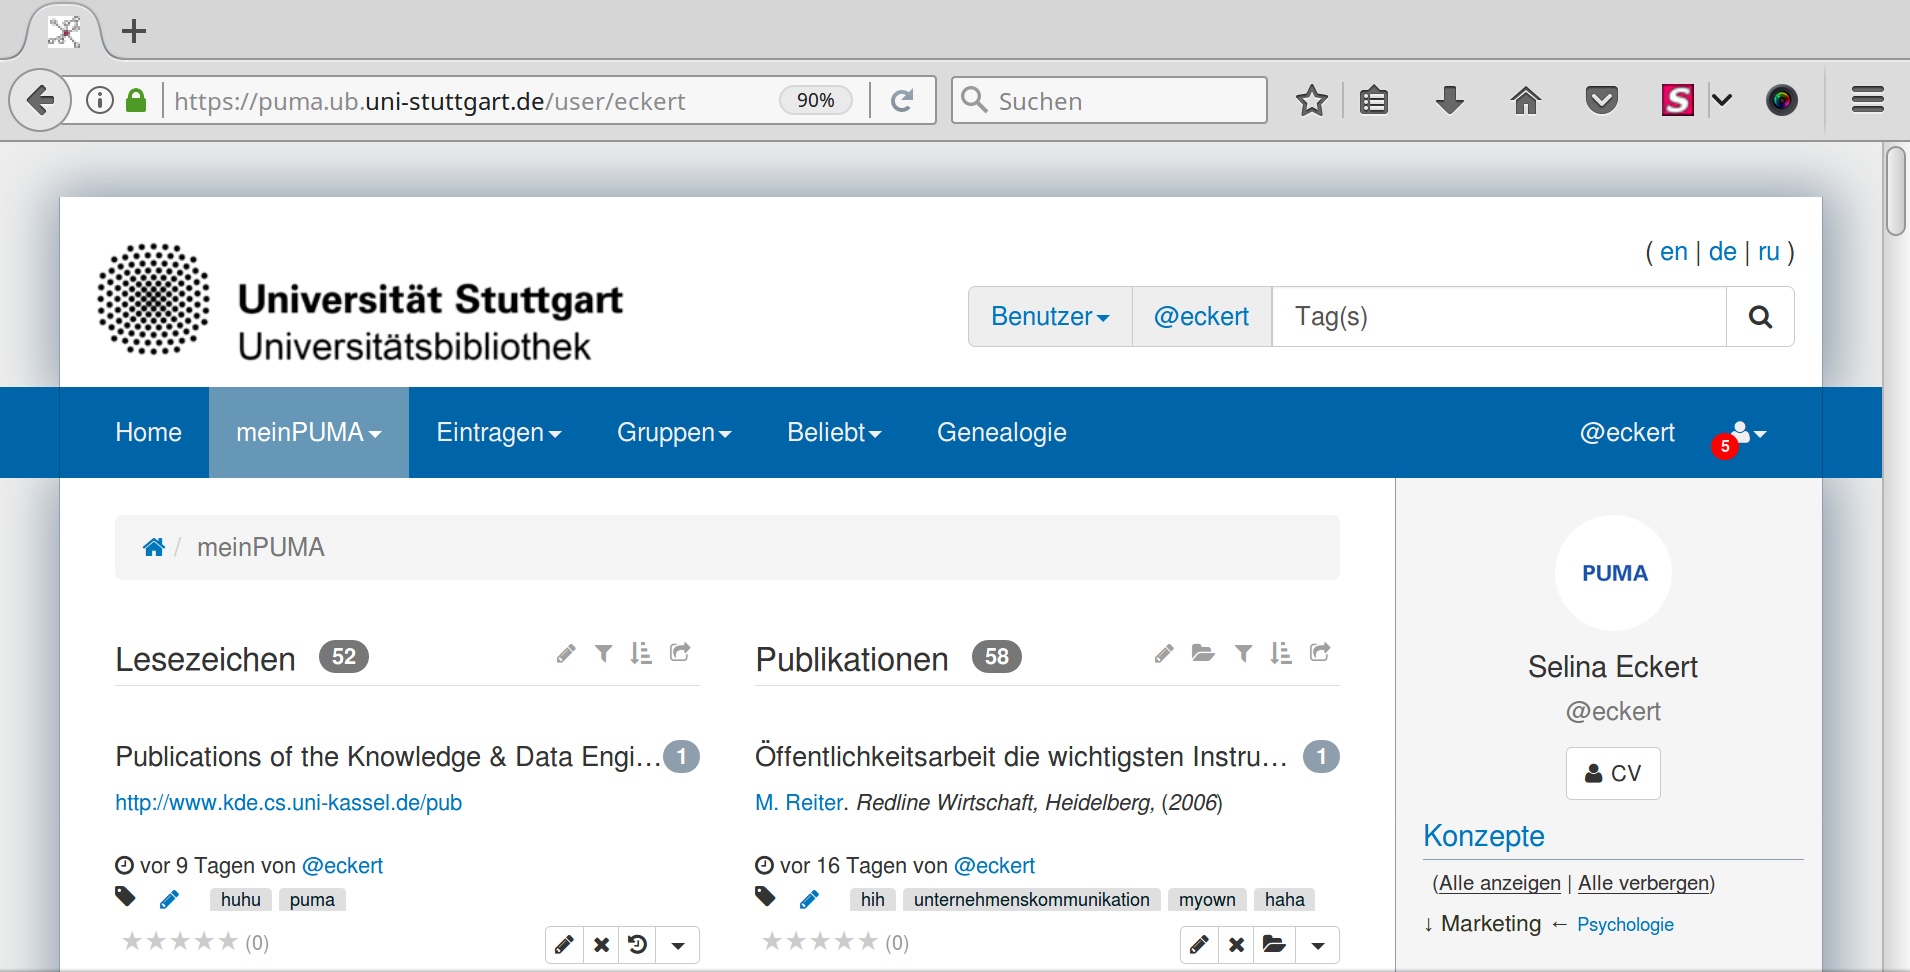
\includegraphics[width=11cm]{Bilder/Kapitel5/CV_Benutzerkonto}}
 \caption{Das Benutzerkonto}
 \label{figure005}
\end{figure}  
Lebenslauf bearbeiten\index{Lebenslauf!bearbeiten}: 
\begin{enumerate}
    \item Klicken Sie auf Ihren Benutzernamen (@username).
    \item Klicken Sie rechts neben Ihrem Profilbild auf den CV-Button.
    \item Ihr Lebenslauf öffnet sich (Ansicht: So wie ihn andere Nutzer sehen).
    \item Um den Lebenslauf zu bearbeiten klicken Sie auf das schwarze Zahnrad neben \enquote{Curriculum Vitae}.
    \item Klicken Sie anschließend im Untermenü auf \enquote{Lebenslauf bearbeiten}. Sie können nun ein vordefiniertes Layout auswählen oder selbst ein Layout mit der MediaWiki-Syntax definieren.
\end{enumerate}
\textbf{Alternativer Weg:} 
\begin{enumerate}
    \item Klicken Sie auf das Personensymbol. Es öffnet sich ein Untermenü.
    \item Klicken Sie im Untermenü auf \enquote{Einstellungen}.
    \item Eine neue Seite öffnet sich. Klicken Sie auf den Reiter \enquote{Lebenslauf}. Sie können nun ein vordefiniertes Layout auswählen oder selber ein Layout mit der MediaWiki-Syntax definieren.
\end{enumerate}
%\begin{wrapfigure}{l}{5cm}
\begin{mdframed}[style=tipp]\texttt{Wenn Sie zwischen den vordefinierten Layouts wechseln, geht Ihr selbst definiertes Layout verloren.} 
\end{mdframed}
%\end{wrapfigure}
\begin{figure}[h!]
 \centering
 \fbox{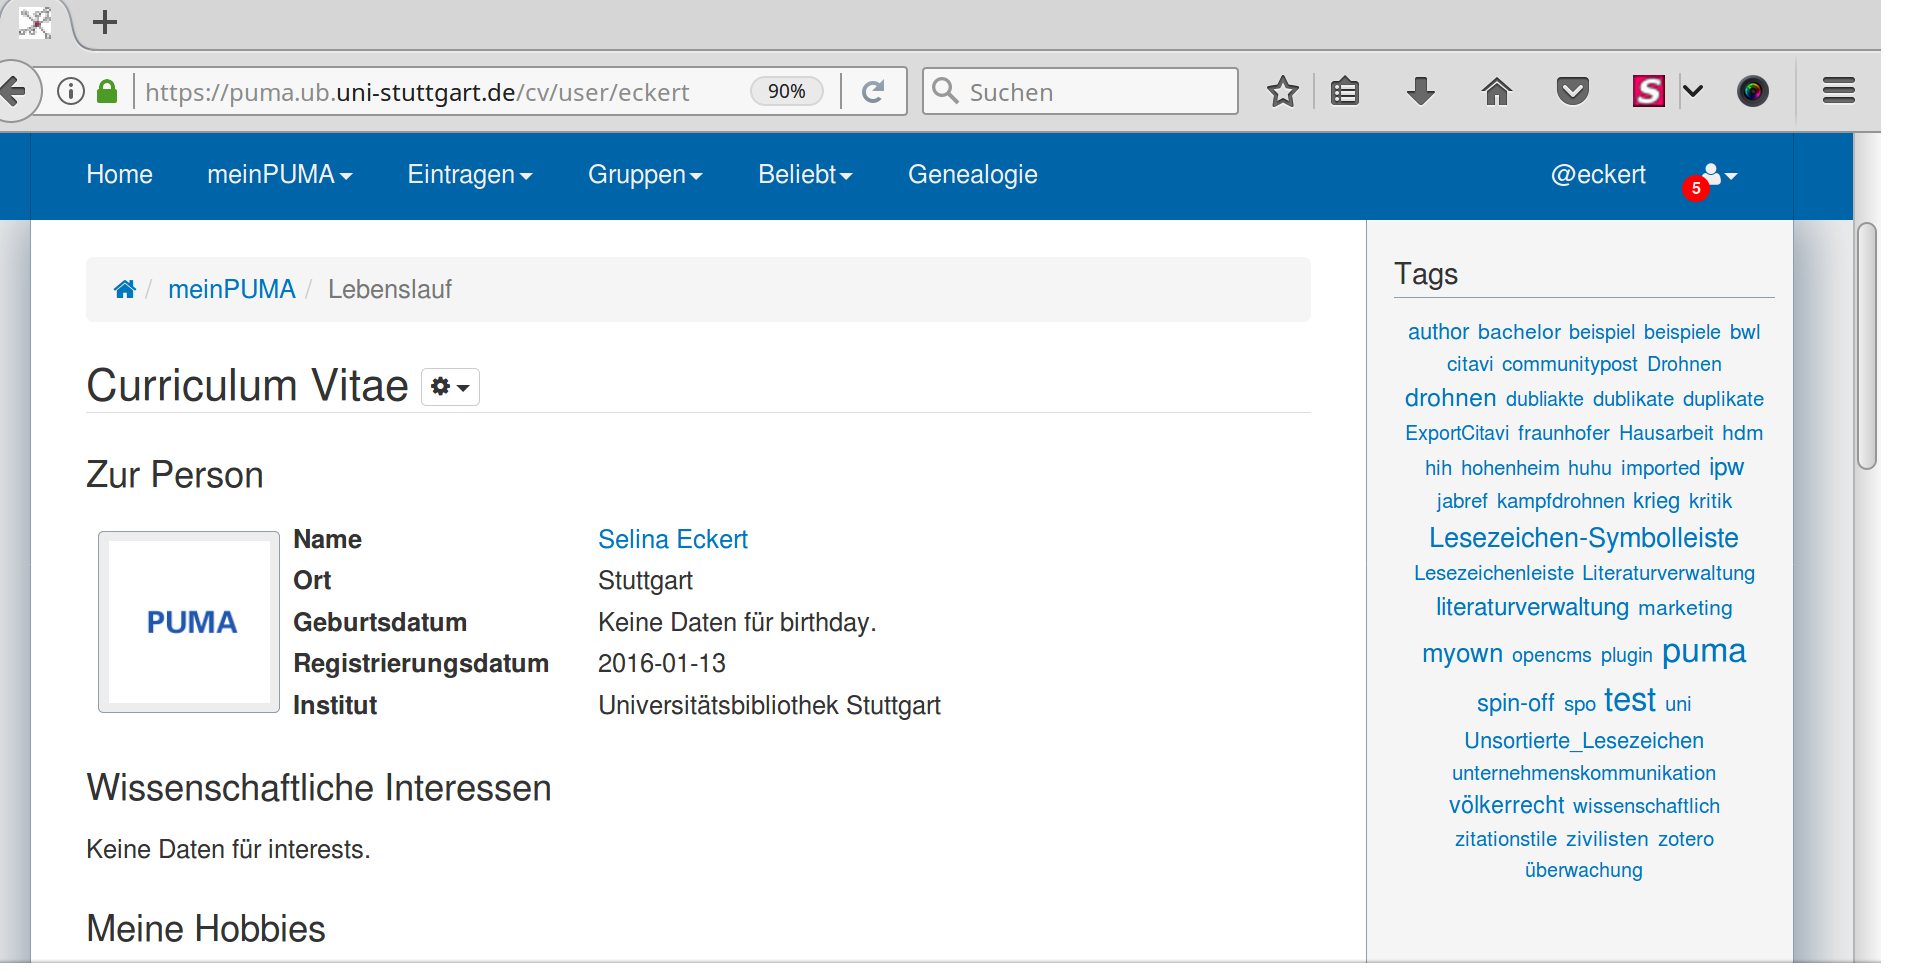
\includegraphics[width=11cm]{Bilder/Kapitel5/CV_Seite}}
 \caption{Curriculum Vitea-Seite}
 \label{figure006}
\end{figure}  
\hypertarget{Eigenes Layout}{Eigenes Layout\index{Lebenslauf!Eigenes Layout}:}
\newline
Um sich selbst ein Layout zu definieren, müssen Sie die MediaWiki-Sytax verwenden. Um Zeit zu sparen bieten wir Ihnen einige XHTML-Tags an: % Tabelle % ist XHTML bei wiki???
\newline
Für die Tags \textit{<publications />} und \textit{<bookmarks />} können Sie außerdem eigene Tags als Ressourcenselektoren benutzen, wenn Sie tags=\enquote{tag1 tag2 (...)} als Attribute anfügen. Beispielsweise liefert \textit{<publications tags=\enquote{data mining} />} alle Ihre Publikationen, die Sie sowohl mit data als auch mit mining getagged haben. 
\begin{figure}[h!]
 \centering
 \fbox{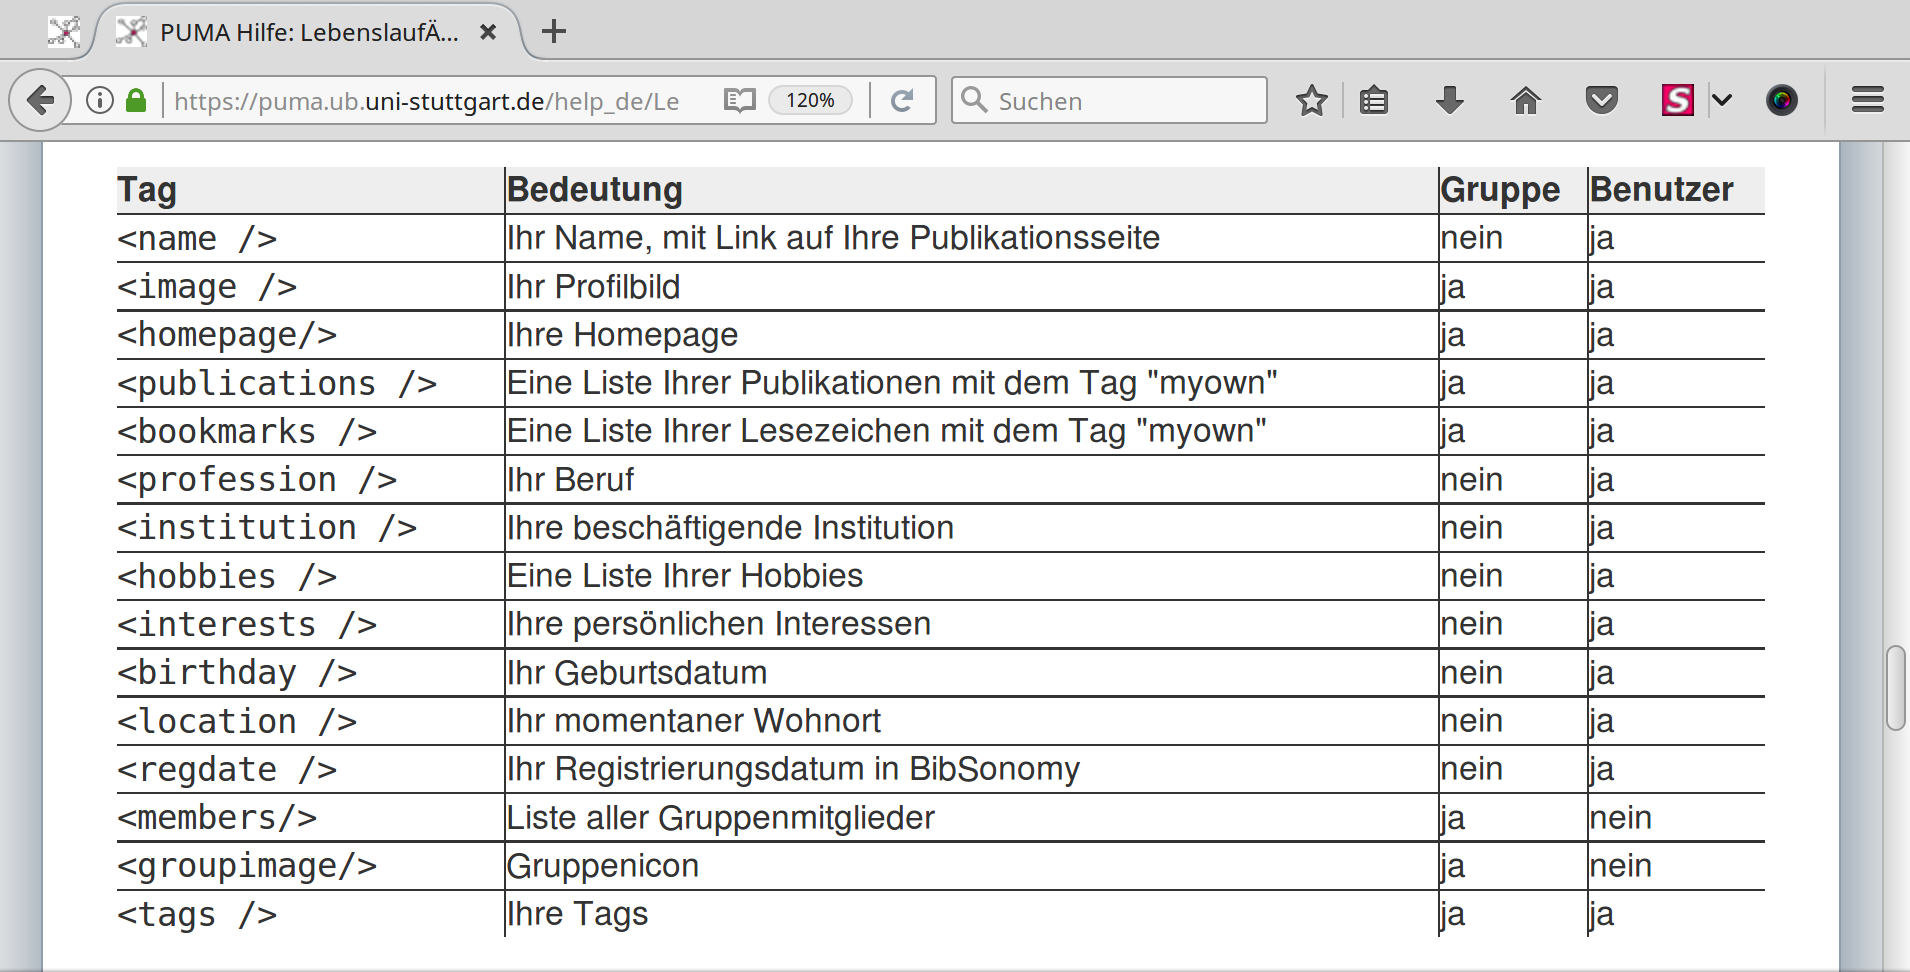
\includegraphics[width=11cm]{Bilder/Kapitel5/xhtml_tags}}
 \caption{XHTML-Tags}
 \label{figure007}
\end{figure}  
\section{Publikationen}
Grundlagen:
\newline
Unter Publikationen\index{Publikationen} versteht man in PUMA alle Arten von Dokumenten (Artikel, Monografie, usw.). Sie können eigene oder fremde Publikationen (z.B. als Basis für eine Literaturrecherche) mit PUMA erstellen/~verwalten/~recherchieren. 
\begin{figure}[h!]
 \centering
 \fbox{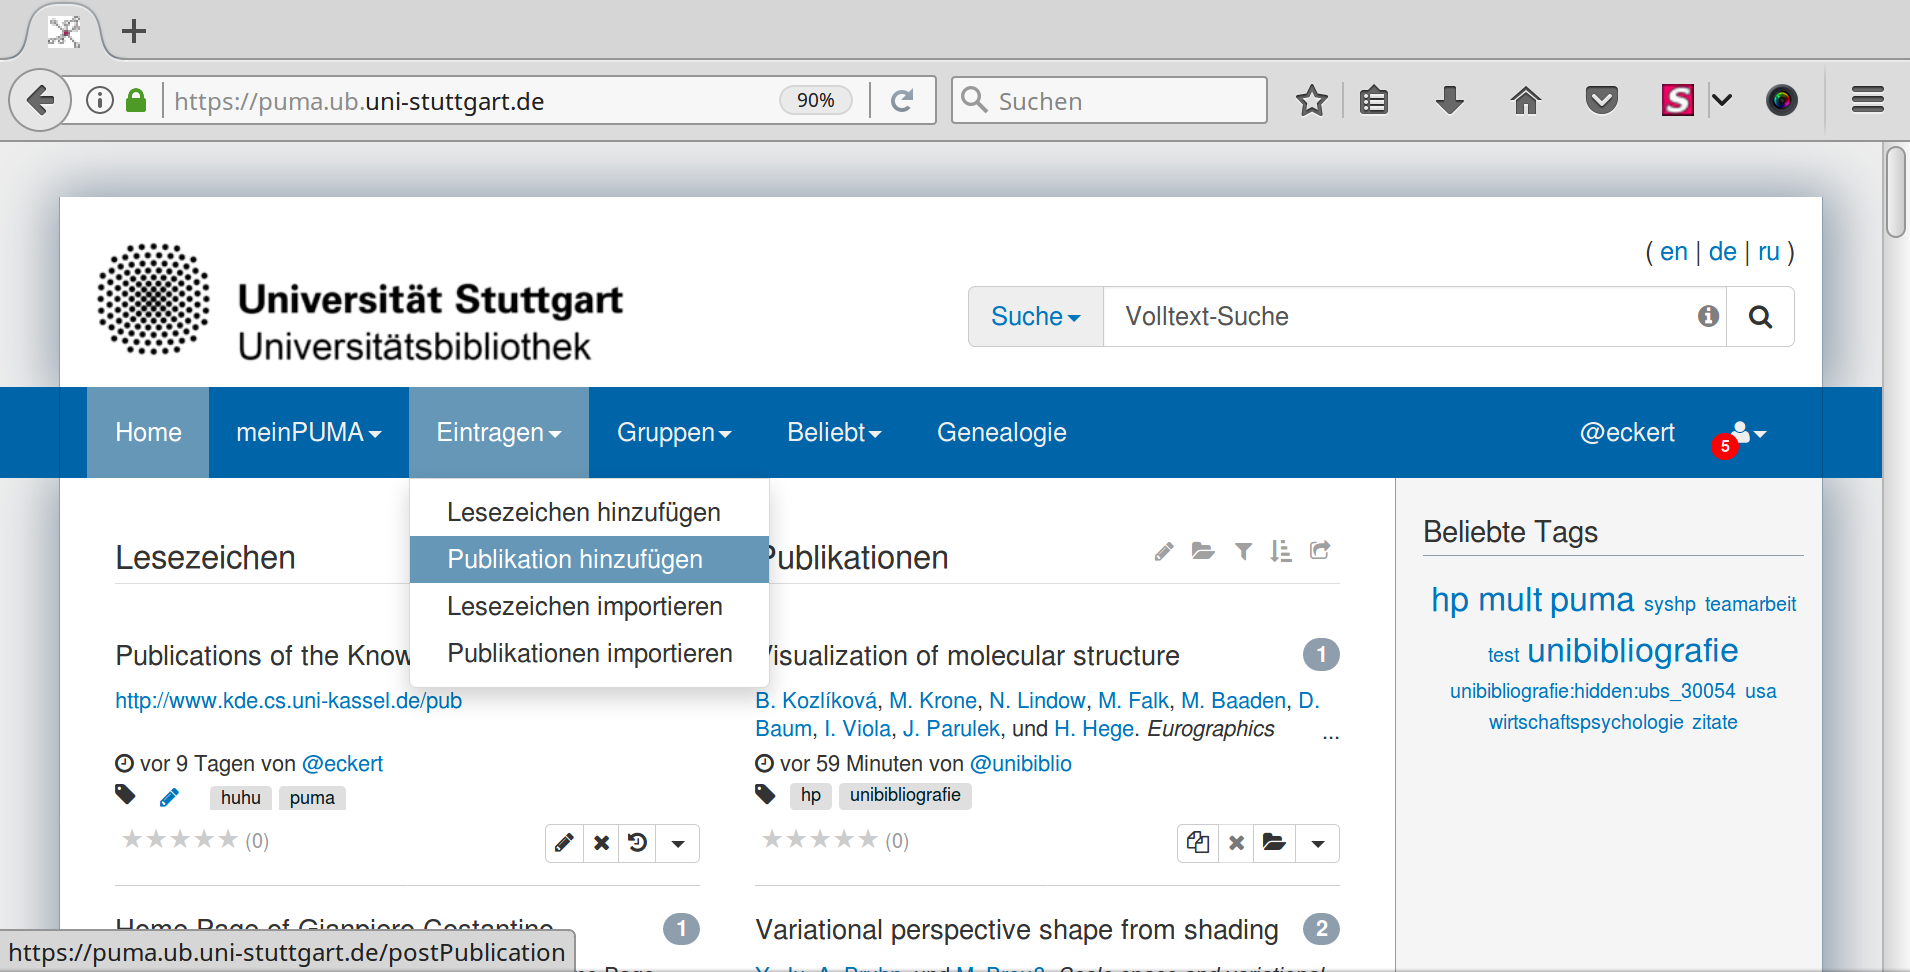
\includegraphics[width=11cm]{Bilder/Kapitel5/Publikation_eintragen}}
 \caption{Publikationen eintragen}
 \label{figure008}
\end{figure}  
Publikationen hinzufügen\index{Publikationen!hinzufügen}:
\begin{enumerate}
    \item Klicken Sie auf den Menüpunkt \enquote{Eintragen} im Hauptmenü. Ein Untermenü klappt auf.
    \item Klicken Sie im Untermenü auf \enquote{Publikation hinzufügen}.
    \item Sie können nun direkt in das Textfeld den Titel oder die ISBN/~ISSN/~DOI der Publikationen eingeben und PUMA zeigt Ihnen die entsprechenden Metainformationen der Publikation an. Neben dieser Weg bietet PUMA Ihnen vier weitere Möglichkeiten Ihre Publikationen einzutragen:
\begin{figure}[h!]
 \centering
 \fbox{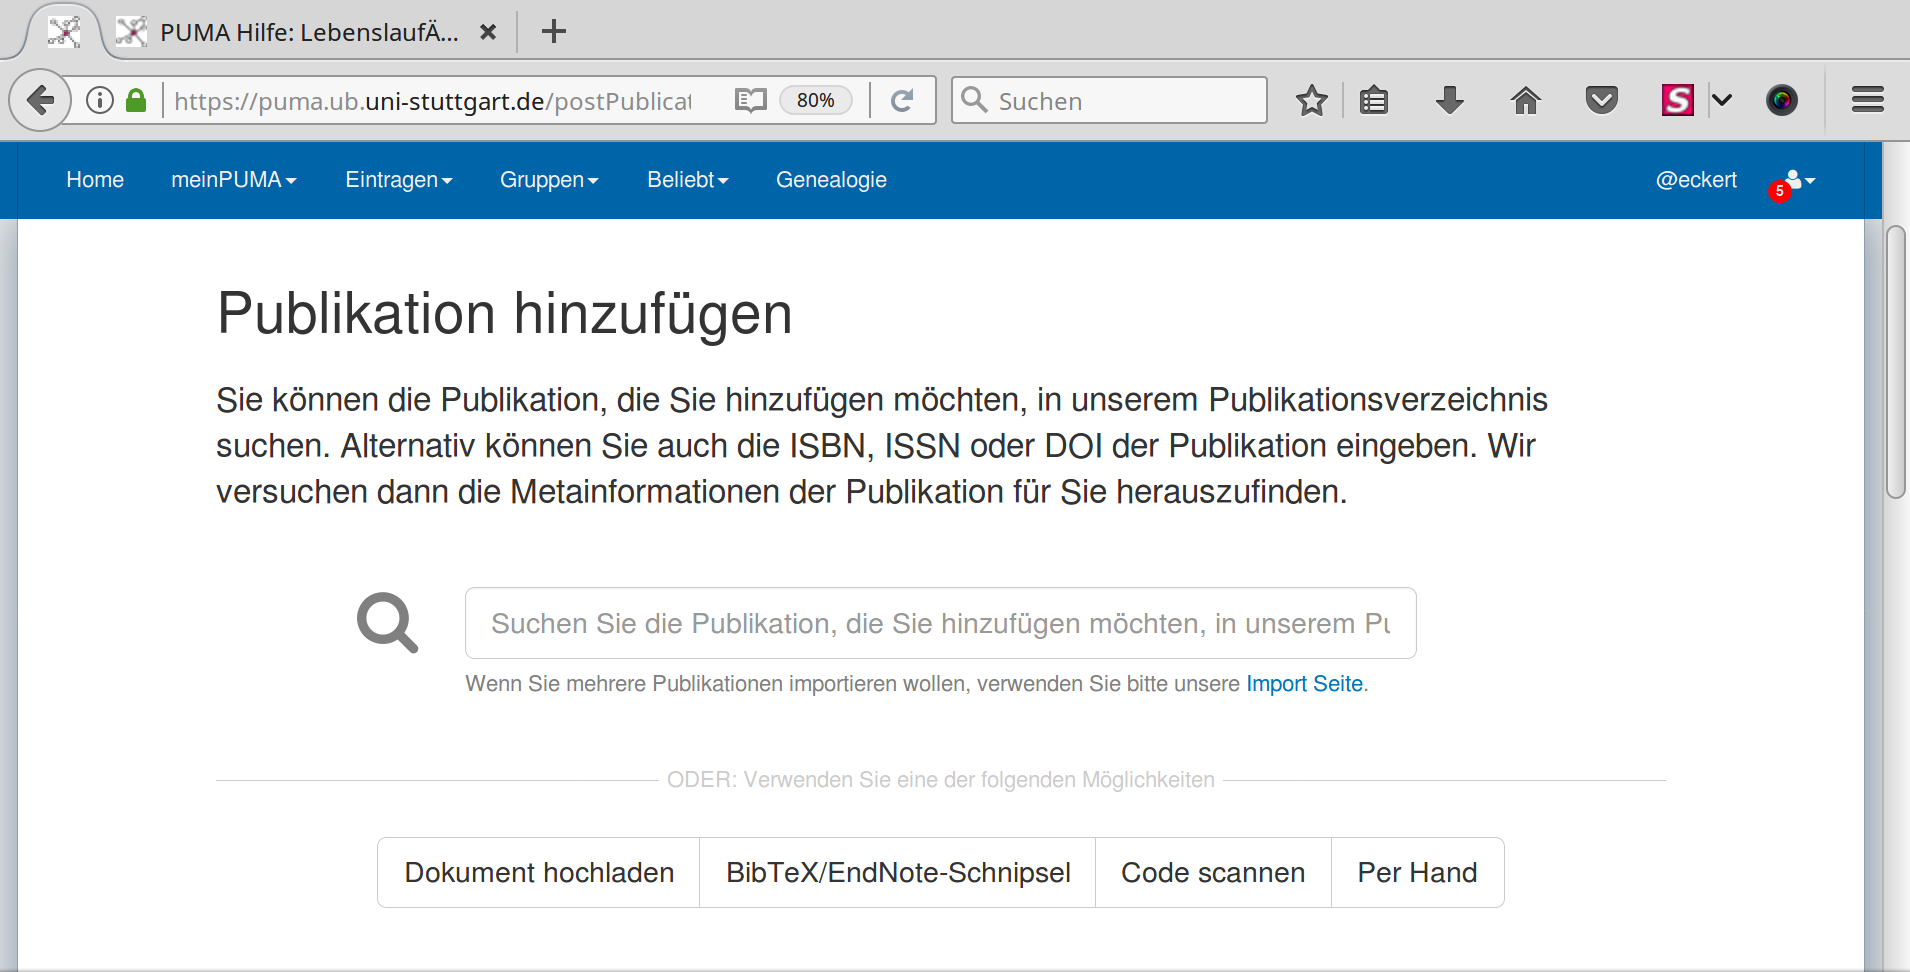
\includegraphics[width=11cm]{Bilder/Kapitel5/Eintragsmoeglichkeiten}}
 \caption{Eintragsmöglichkeiten}
 \label{figure009}
\end{figure}  
    \begin{itemize}
    	\item Dokument hochladen:\newline
        Voraussetzung ist, dass es sich um eine BibTex- oder EndNote-Datei handelt.
        \begin{enumerate}
            \item Klicken Sie auf \enquote{Datei hochladen}.
            \item Über den \enquote{Durchsuchen} Button haben Sie die Möglichkeit die gewünschte Datei auszuwählen.
            \item Der Dateiname, der ausgewählten Datei, erscheint hinter dem Durchsuchen-Button. Sie können anschließend die Sichtbarkeit des Eintrags festlegen. Durch das Klicken auf \enquote{Speichern} erhalten Sie die Detailansicht der Publikation und können diese nochmals überarbeiten und auf ihre Richtigkeit überprüfen.
            \item Klicken Sie anschließend nochmals auf \enquote{Speichern} um die Publikation in Ihre Sammlung einzutragen.
        \end{enumerate}
        \item BibTex\index{BibTex}/EndNote\index{EndNote}-Schnipsel:
        \newline
        Voraussetzung ist, dass Sie Ihre Literaturliste aus Ihrem bisherigen Literaturverwaltungsprogramm in die Zwischenablage exportieren.
        \begin{enumerate}
            \item Klicken Sie auf den Reiter \enquote{BibTex/EndNote-Schnipsel}.
            \item Fügen Sie den Text aus der Zwischenablage in das Textfeld \enquote{Auswahl} ein. Dies können Sie so erreichen, indem Sie auf das Textfeld Auswahl gehen und mit der rechte Maustaste das Menü öffnen und auf \enquote{Einfügen} klicken. Erscheint das Wort \enquote{Einfügen} grau, dann haben Sie keine Daten in die Zwischenablage exportiert und Sie müssen den Text erneut in die Zwischenablage einfügen.
            \item Klicken Sie auf \enquote{Weiter}.
            \item PUMA zeigt Ihnen nun eine Übersicht über alle Daten an. Überprüfen Sie diese auf ihre Richtigkeit.
            \item Klicken Sie \enquote{Speichern}.
        \end{enumerate}
        \item Code scannen\index{Code Scannen}: 
        \newline
        Voraussetzung ist, dass Sie über eine eingebaute Webcam verfügen oder eine externe Webcam anschließen, bevor Sie mit der Aufnahme beginnen können.
        \begin{enumerate}
            \item Klicken Sie auf den Reiter \enquote{Code scannen}. Es kann passieren, dass Ihr Webbrowser eine Warnmeldung anzeigt, dass die Webseite (PUMA) versucht auf Ihre Webcam zuzugreifen. Falls dies der Fall sein sollte, erlauben Sie den Zugriff.
            \item Das Bild der Webcam erscheint auf Ihrem Bildschirm. Halten Sie den Strichcode ruhig und gut sichtbar vor Ihre Webcam. Sobald PUMA den ISBN-Strichcode erkennt, ertönt ein Kamerageräusch.
            \item Wenn der Strichcode erkannt wurde, werden die Daten automatisch angezeigt. Überprüfen Sie diese auf ihre Richtigkeit und klicken Sie anschließend auf \enquote{Speichern}.
        \end{enumerate}
\begin{figure}[h!]
 \centering
 \fbox{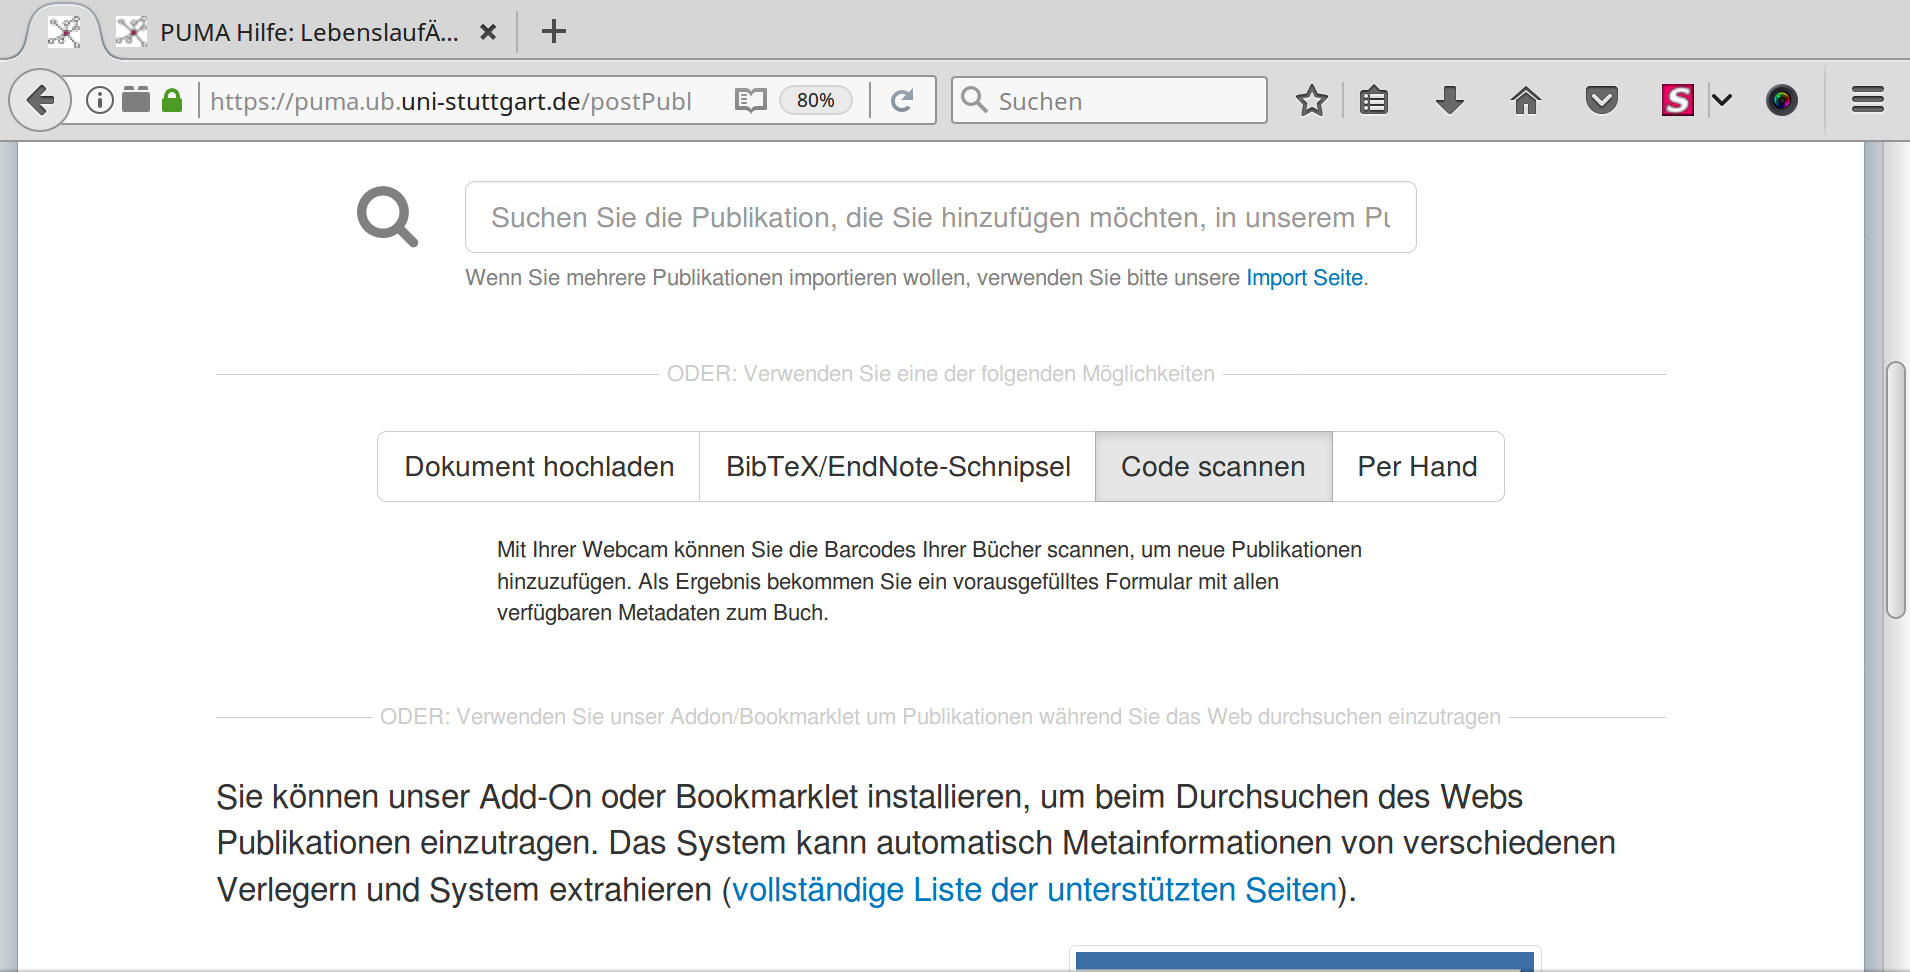
\includegraphics[width=11cm]{Bilder/Kapitel5/Code_scannen}}
 \caption{Code scannen}
 \label{figure010}
\end{figure}  
        \item Per Hand:
        \begin{enumerate}
            \item Klicken Sie auf den Reiter \enquote{Per Hand}.
            \item Geben Sie alle geforderten Daten in die entsprechenden Felder ein und klicken Sie anschließend auf \enquote{Weiter}. 
            \item Im nächsten Schritt können Sie weiterführende Informationen angeben. Sie können aber auch gleich auf \enquote{Speichern} klicken, um die Publikation einzutragen.
        \end{enumerate}        
    \end{itemize}
\end{enumerate}
\section{Lesezeichen} % 2Screenshots: Anfang+Möglichkeiten
Grundlagen:
\newline
Lesezeichen\index{Lesezeichen} (engl. Bookmark) ermöglichen es, das Internet wie ein Buch zu verwenden. Mit einem Lesezeichen merken Sie sich die genaue Adresse eines Internet-Dokuments. PUMA gibt Ihnen die Möglichkeit Lesezeichen zentral zu speichern, zu verwalten und auf sie zuzugreifen. 
\newline
\newline
Lesezeichen hinzufügen\index{Lesezeichen!hinzufügen}: 
\begin{figure}[h!]
 \centering
 \fbox{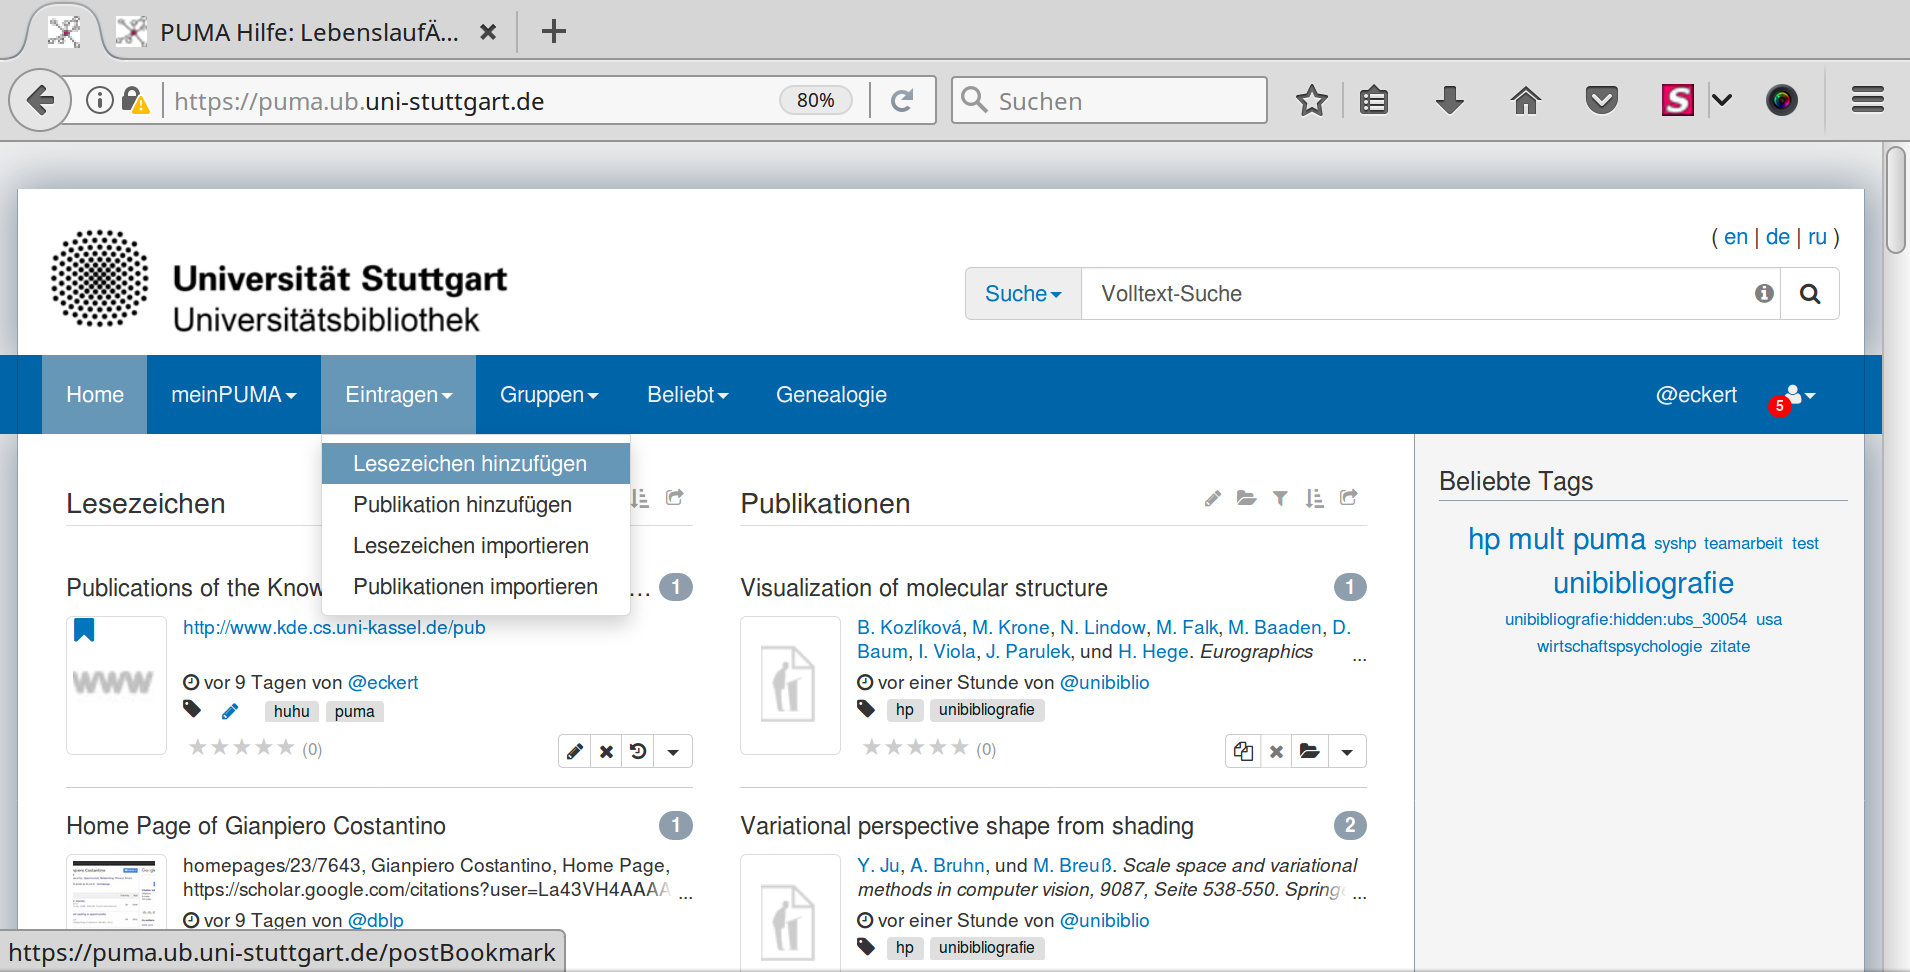
\includegraphics[width=11cm]{Bilder/Kapitel5/Lesezeichen_hinzufuegen}}
 \caption{Lesezeichen hinzufügen}
 \label{figure011}
\end{figure} 
\begin{enumerate}
    \item Klicken Sie auf den Menüpunkt \enquote{Eintragen}\index{Lesezeichen!eintragen} im Hauptmenü. Ein Untermenü klappt auf.
    \item Klicken Sie im Untermenü auf \enquote{Lesezeichen hinzufügen}.
    \item Tragen Sie in das Feld \enquote{URL} die Adresse (URL) der Webseite ein, die Sie als Lesezeichen hinzufügen möchten. Anschließend klicken Sie auf \enquote{Weiter}. 
    \item Im Folgenden werden Sie aufgefordert einige Zusatzdaten einzugeben:
    \begin{itemize}
        \item URL: Wird automatisch aus dem Schritt davor übernommen.
        \item Titel: Tragen Sie den Titel der Seite ein. 
        \item Beschreibung/~Kommentar: Hier können Sie eigene Kommentare zum Lesezeichen hinterlegen. 
			%\begin{wrapfigure}{r}{5cm}
			\begin{mdframed}[style=tipp]\texttt{In diesem Feld können Sie z. B. auch ein kleines Abstract hinterlegen.} 
			\end{mdframed}
			%\end{wrapfigure}
        \item Tags: Tags\index{Tags} (dt. Schlagwörter) ermöglichen ein übersichtliches Organisieren und Strukturieren der Lesezeichen. Sie können so viele Tags verwenden, wie Sie wollen. Die einzelnen Tags werden durch Leerzeichen von einander getrennt. \newline 
        	%\begin{wrapfigure}{r}{5cm}
        	\begin{mdframed}[style=tipp]
	\texttt{Wenn Sie einen Tag verwenden möchten, der aus mehreren Worten besteht (z.~B. Fachbereich Architektur) dann verwenden Sie PascalCase, z.~B. FachbereichArchitektur.} 
			\end{mdframed}
			%\end{wrapfigure}
        \item Sichtbarkeit: Legen Sie fest, wer Ihr Lesezeichen sehen darf. Sie können wählen zwischen öffentlich\index{Sichtbarkeit!öffentlich} (alle Nutzer), privat\index{Sichtbarkeit!privat} (nur Sie selbst) oder andere\index{Sichtbarkeit! andere} (Freunde oder eine Gruppe). Außerdem können Sie bei \enquote{Interessant für} eine spezielle Gruppe auf Ihr Lesezeichen aufmerksam machen.  
    \end{itemize}
    \item Klicken Sie abschließend auf \enquote{Speichern} um das Lesezeichen einzutragen. Das Lesezeichen ist nun gespeichert. Bitte beachten Sie, dass ein neues Lesezeichen bei der Suchanfrage ein bisschen Zeit benötigt (1 Sekunde bis weniger als eine Minute). 
\end{enumerate}
\underline{Wichtig bei der Recherche und Archivierung von Lesezeichen:}
\begin{itemize}
    \item Puma speichern nicht das eigentliche Dokument, sondern nur die Adresse des Internet-Dokuments. Es kann somit passieren, dass ein Dokument zu einem späteren Zeitpunkt nicht mehr abrufbar ist, da z.B. sich die Adresse geändert hat oder es gelöscht wurde.  Aus diesem Grund ist es nützlich, dass Sie sich ein Sicherheitskopie des Dokuments anlegen und diese auf Ihrem Computer speichern.
    \item Neben den oben genannten Punkten bitten wir Sie auch darum zu bedenken, dass ein Internet-Dokument jederzeit geändert werden kann. Aus diesem Grund empfiehlt sich hier ebenfalls eine Sicherungskopie. 
    \item Zudem sollten Sie beachten, dass in der Literaturangabe zu einem Internet-Dokument IMMER das Datum und die Uhrzeit des letzten Abrufs mit angegeben werden muss. Dies entspricht den allgemeinen Richtlinien wissenschaftlichen Arbeitens. Diese Angaben können Sie in das Feld Beschreibung/~Kommentar eintragen.
    \item PUMA unterstützt die RFC 7089\footnote{\url{http://tools.ietf.org/html/rfc7089}} Spezifikation\index{RFC 7089 Spezifikation}. Damit wird es möglich, Lesezeichen so zu betrachten, wie sie in PUMA gespeichert wurden, selbst wenn sich die Seite in der Zwischenzeit geändert hat. Um diese Funktion zu nutzen, müssen Sie das Memento-Plugin in ihrem Browser installieren. Das Plugin existiert für Mozilla Firefox\footnote{\url{https://addons.mozilla.org/de/firefox/addon/mementofox/}} und Google Chrome\footnote{\url{https://chrome.google.com/webstore/detail/memento-time-travel/jgbfpjledahoajcppakbgilmojkaghgm?hl=en&gl=US}}. 
\end{itemize}
\section{Versionierung der Publikationen und Lesezeichen}
Publikationen und Lesezeichen können jederzeit eingetragen und bearbeitet werden. Um sich einen Überblick über die vorgenommen Änderungen zu verschaffen, bietet PUMA eine Versionsgeschichte\index{Versionierung} zu jeder Publikation und jedem Lesezeichen an. Klicken Sie in Ihrer eigenen Sammlung auf den kleinen schwarzen Pfeil neben einer beliebigen Publikation. Es öffnet sich ein Dropdown-Menü, in dem Sie \enquote{Verlauf dieser Publikation} auswählen. Ihnen wird sofort die Versionsgeschichte der jeweiligen Publikation/~Lesezeichen angezeigt und Sie können jede Ihrer Änderungen nachverfolgen. 
\begin{figure}[h!]
 \centering
 \fbox{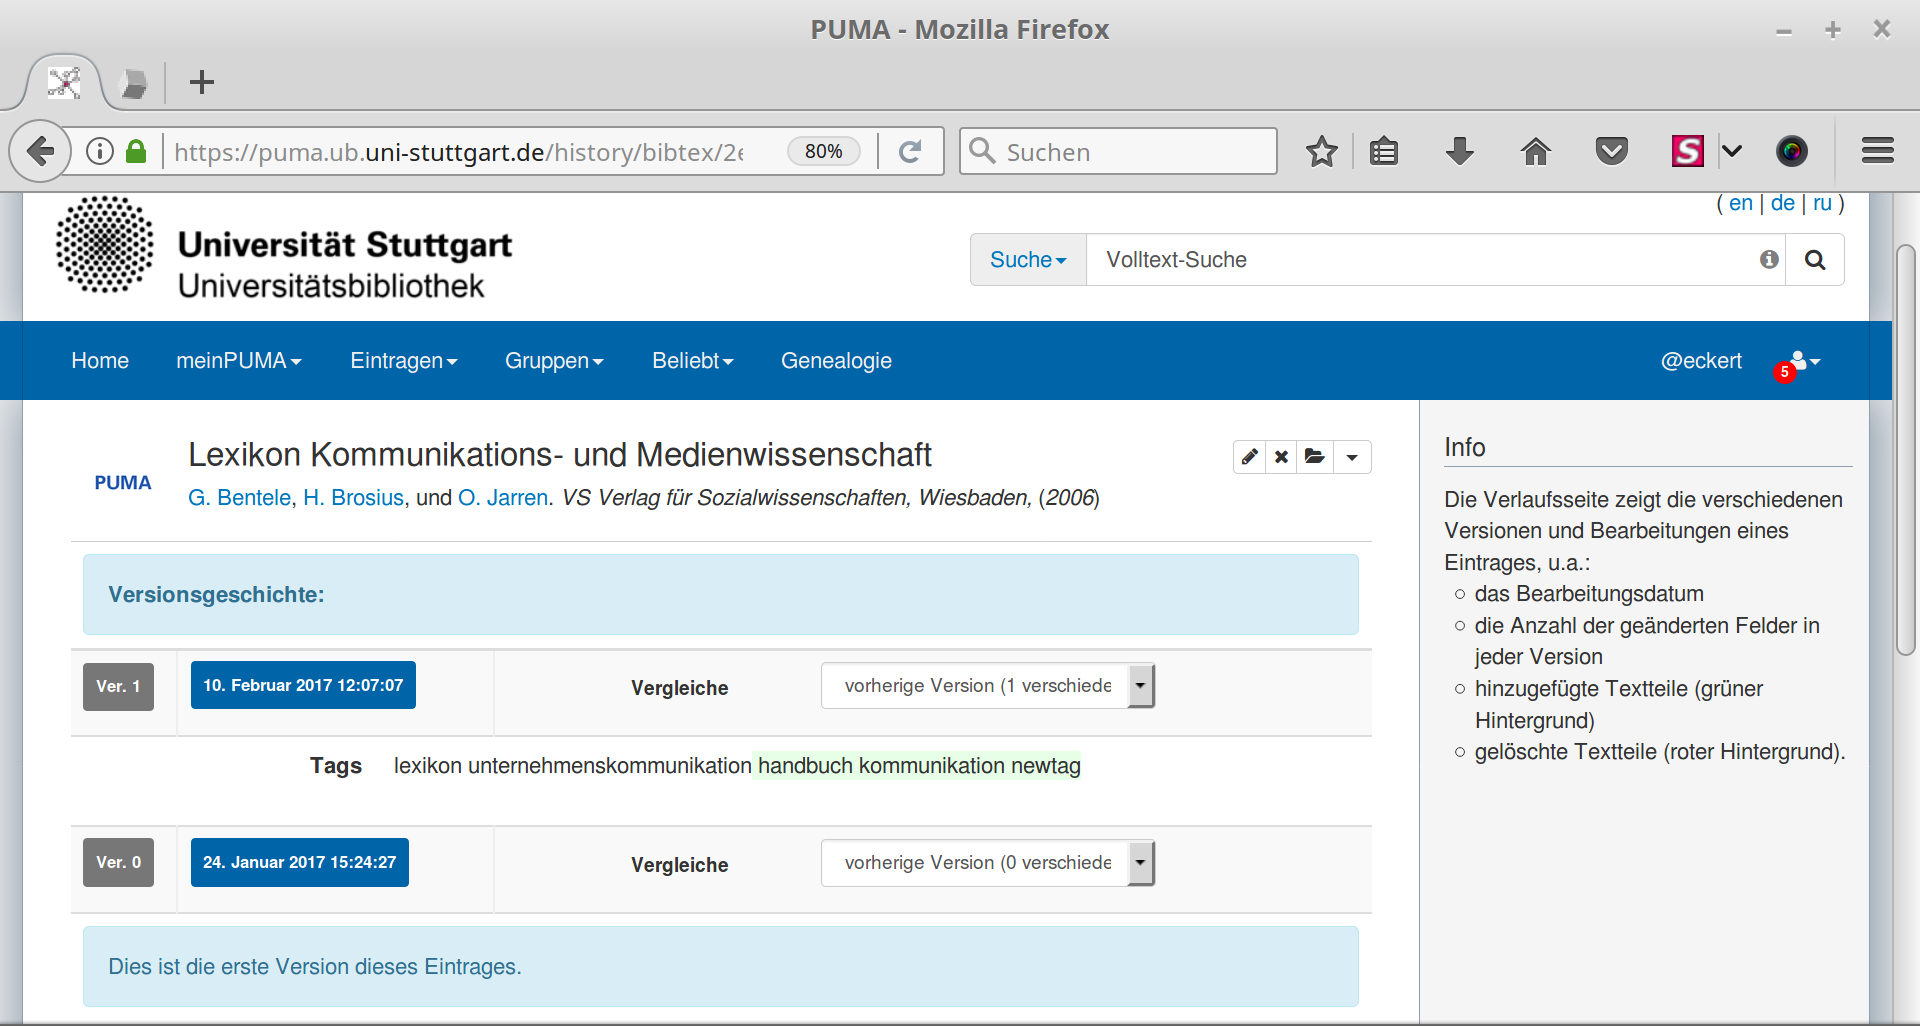
\includegraphics[width=9cm]{Bilder/Kapitel5/Versionsgeschichte}}
 \caption{Die Versionsgeschichte}
 \label{figure012}
\end{figure} 
\section{Lesezeichen importieren}
\subsection{Browser}
PUMA ermöglicht es Ihnen HTML-Dateien in PUMA zu importieren. Hierfür exportieren Sie ihre Lesezeichen aus ihrem Browser als HTML-Datei und importieren diese anschließend. Je nach Browser unterscheidet sich das Exportieren der Lesezeichen.
\newline
\newline
\textbf{Chrome}%Screenshots hab ich schon
\newline Um ihre Lesezeichen in Chrome\index{Chrome} als HTML-Datei zu exportieren, klicken Sie im Menü oben rechts auf \enquote{Lesezeichen} und anschließend auf \enquote{Lesezeichen-Manager}. Es öffnet sich ein neues Fenster, in dem Sie auf \enquote{Organisieren} klicken und im Dropdown-Menü \enquote{Lesezeichen in HTML-Datei exportieren...} wählen. Speichern Sie die Datei ab und fahren mit Schritt 1 von HTML-Datei in PUMA importieren fort, um Ihre Lesezeichen endgültig nach PUMA zu importieren.  
\begin{figure}[h!]
 \centering
 \fbox{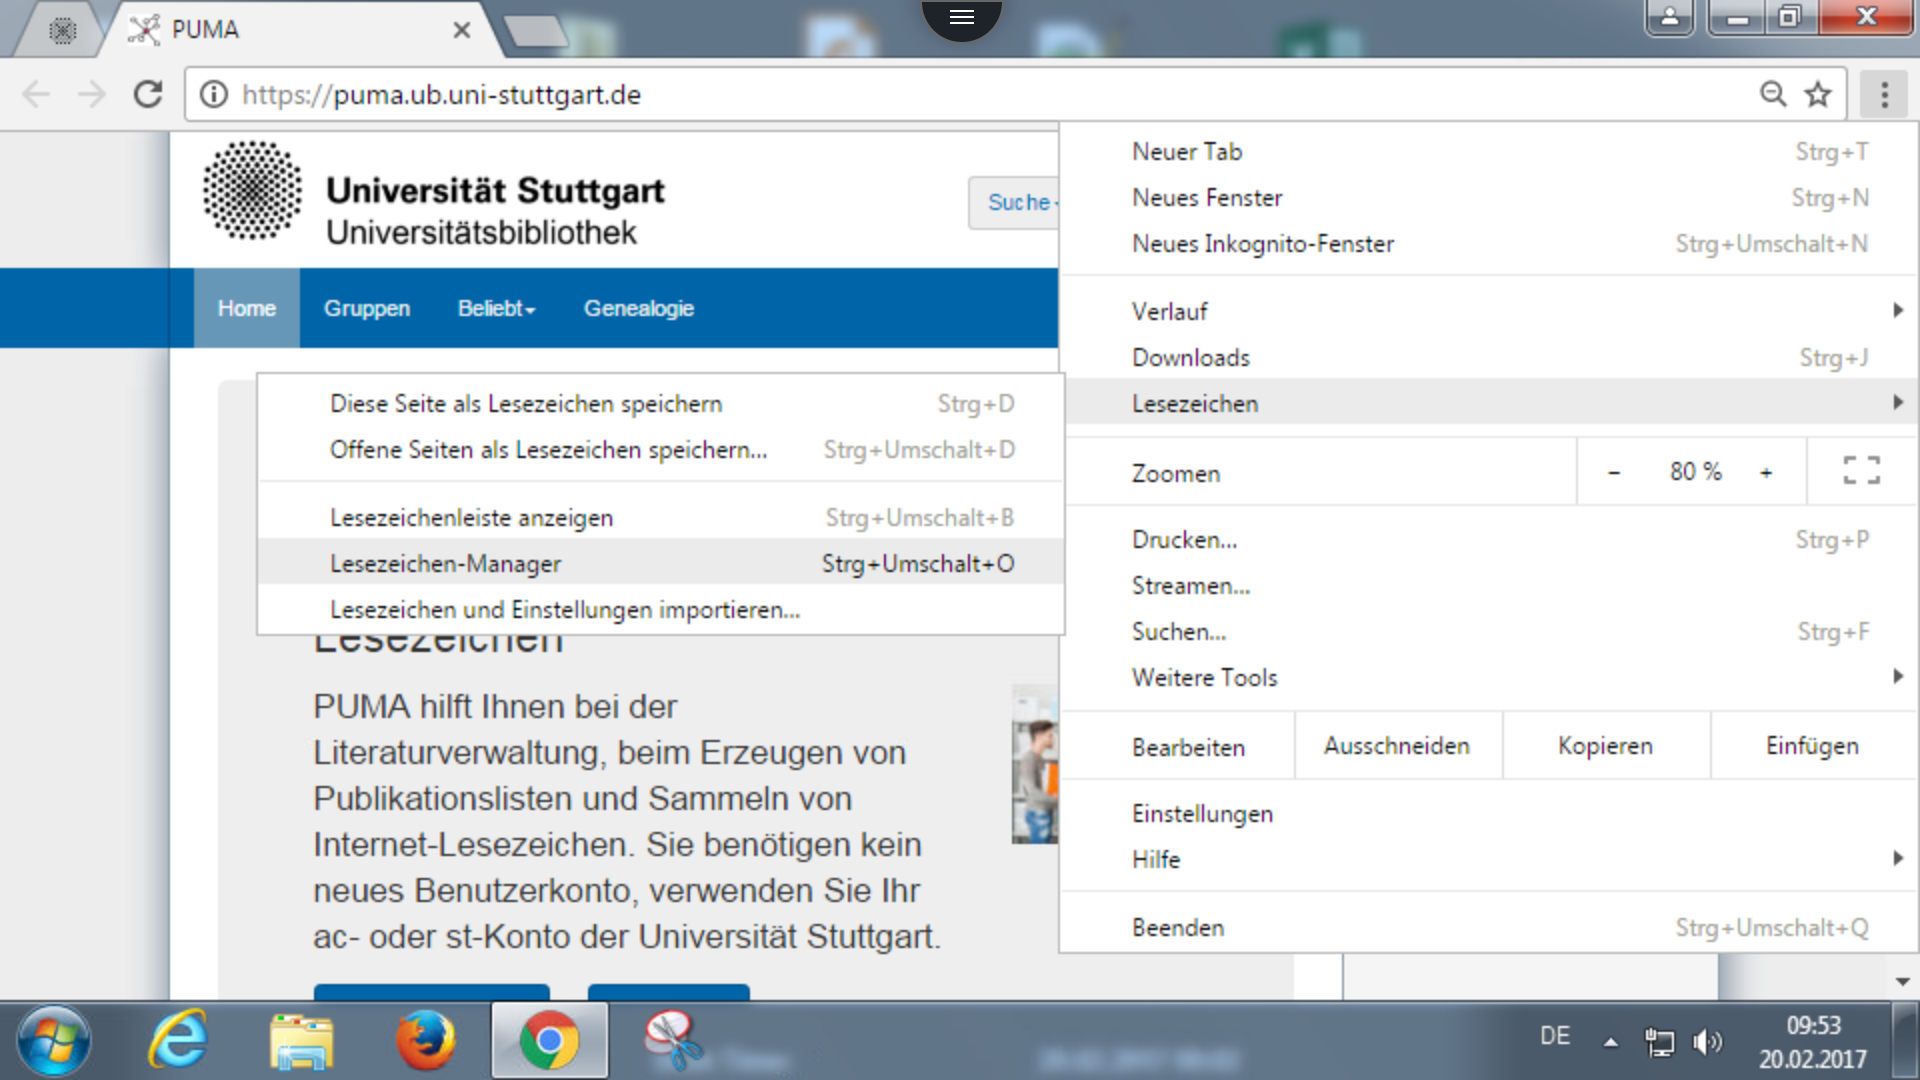
\includegraphics[width=11cm]{Bilder/Kapitel5/Lesezeichen-Manager_Chrome}}
 \caption{Der Lesezeichen-Manager}
 \label{figure013}
\end{figure}
\begin{figure}[ht]
 \centering
 \fbox{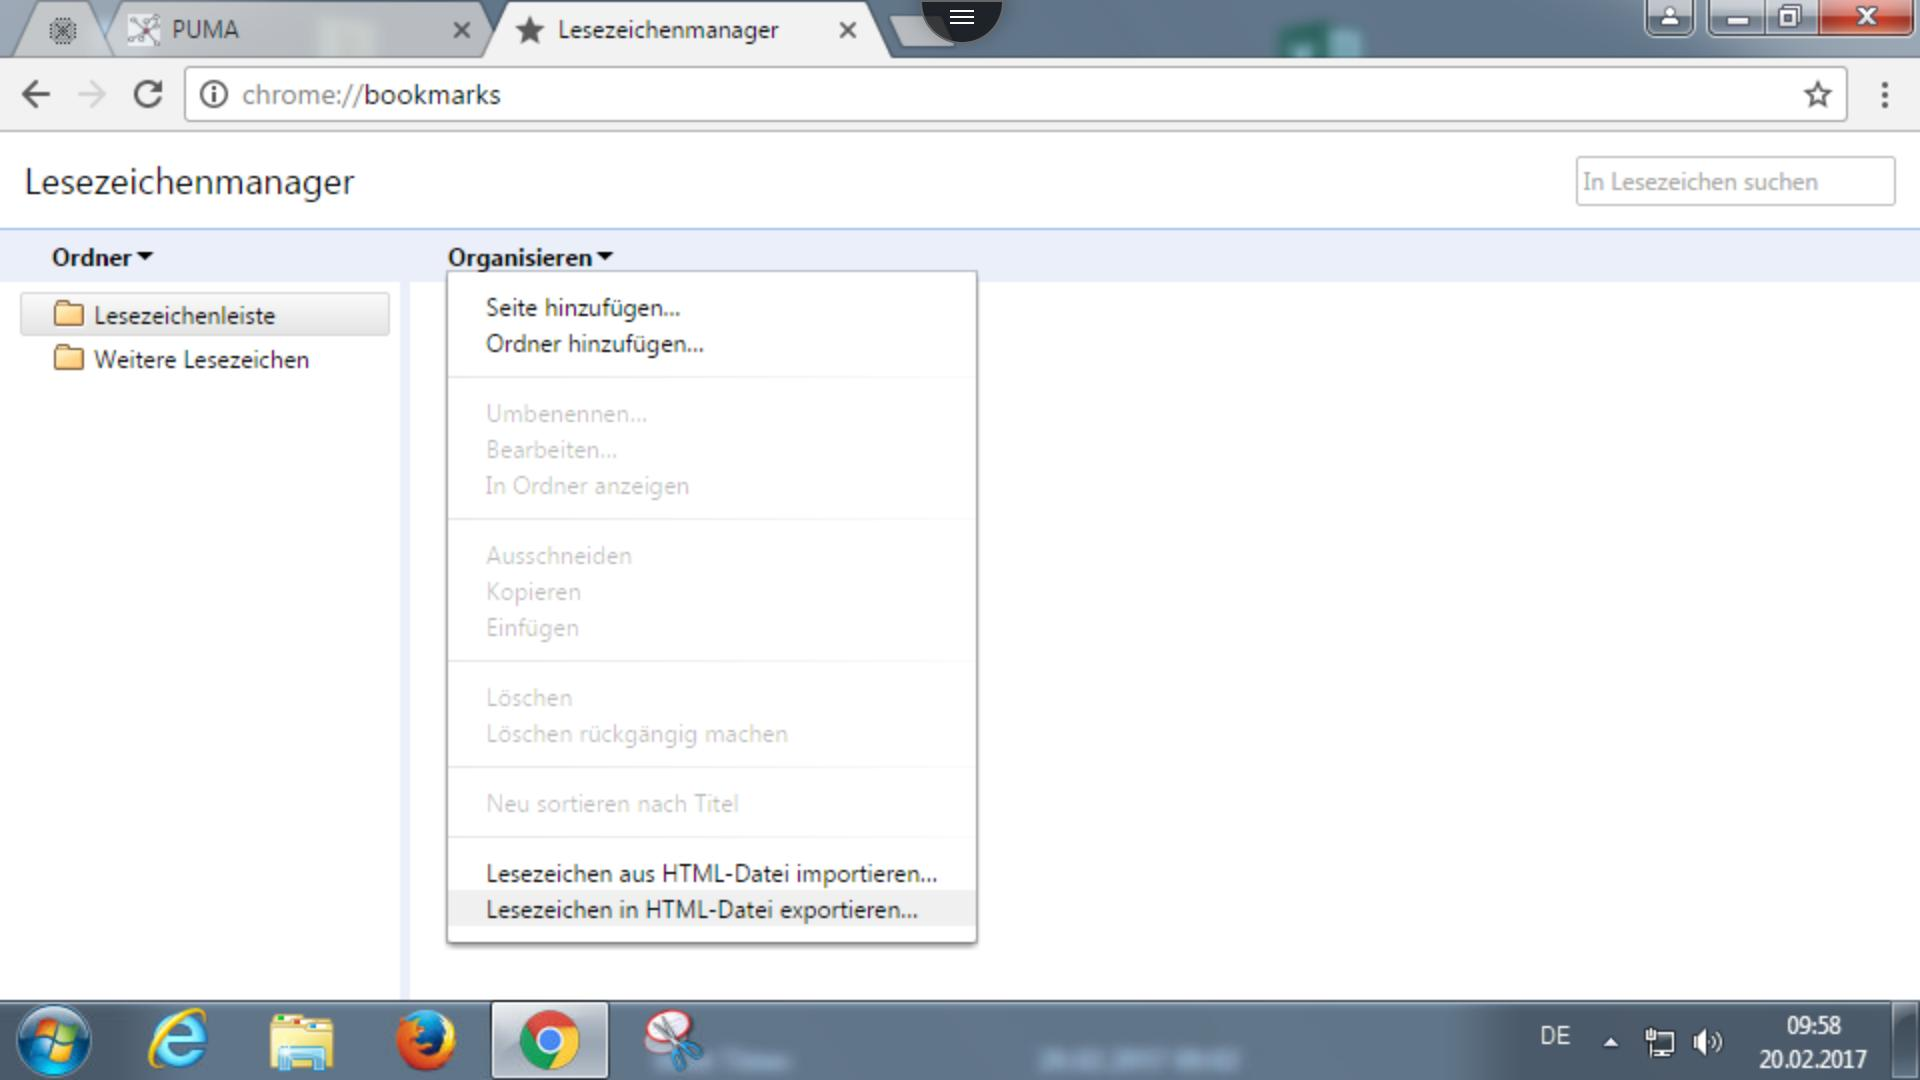
\includegraphics[width=9cm]{Bilder/Kapitel5/Lesezeichen_HTML_Chrome}}
 \caption{Lesezeichen in HTML-Datei exportieren}
 \label{figure014}
\end{figure}

\textbf{Firefox}
\newline Um Ihre Lesezeichen in Firefox\index{Firefox} als HTML-Datei zu exportieren, klicken Sie auf das Lesezeichensymbol rechts neben der Suchleiste. Wählen Sie im Dropdown-Menü \enquote{Lesezeichen verwalten} aus.

\begin{figure}[h!]
 \centering
 \fbox{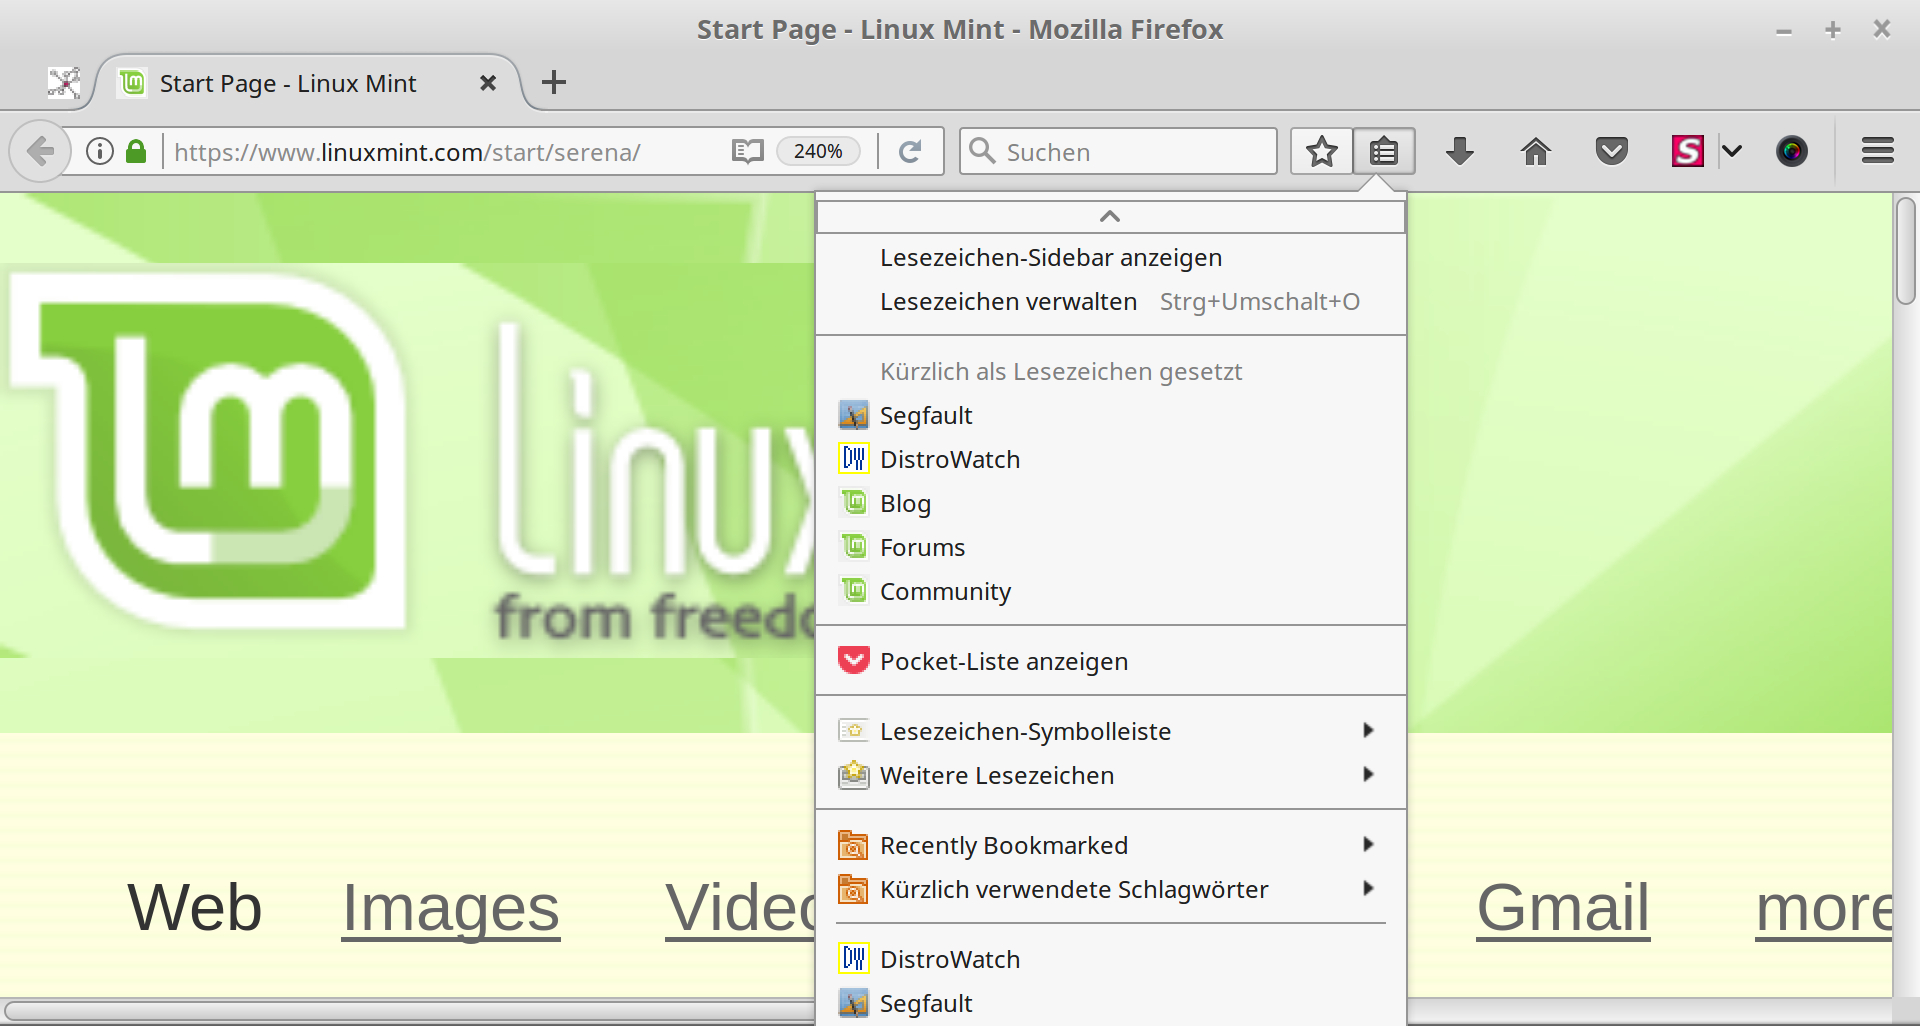
\includegraphics[width=11cm]{Bilder/Kapitel5/Firefox_Lesezeichen_verwalten}}
 \caption{Lesezeichen verwalten}
 \label{figure015}
\end{figure}
Anschließend klicken Sie auf \enquote{Importieren und Sichern} und wählen \enquote{Lesezeichen nach HTML exportieren} aus. Speichern Sie die Datei ab und fahren mit Schritt 1 von HTML-Datei in PUMA importieren fort, um Ihre Lesezeichen endgültig nach PUMA zu importieren.  

\begin{figure}[h!]
 \centering
 \fbox{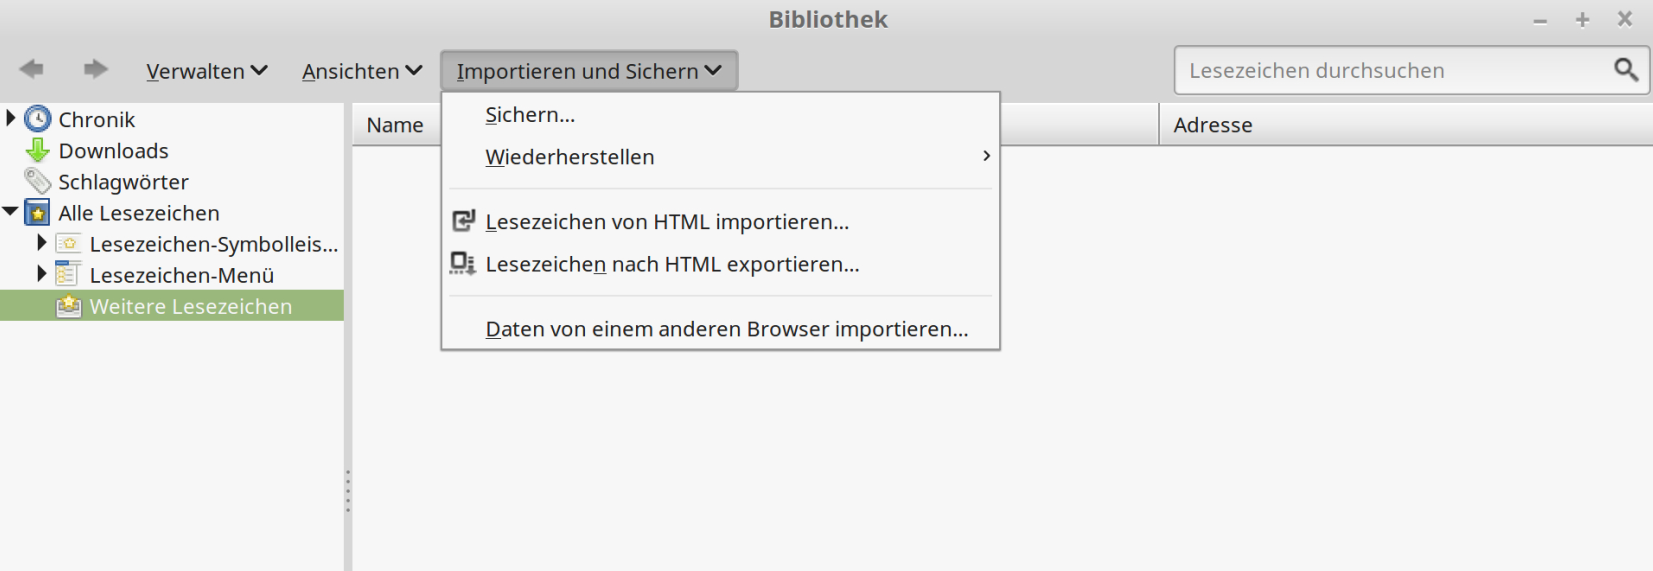
\includegraphics[width=11cm]{Bilder/Kapitel5/Firefox_Importieren_Speichern}}
 \caption{Importieren und Sichern}
 \label{figure016}
\end{figure}
\subsection{HTML-Datei\index{HTML-Datei} in PUMA importieren}
\begin{enumerate}
    \item Klicken Sie auf \enquote{Eintragen} und wählen im Dropdown-Menü \enquote{Lesezeichen importieren} aus.
    \item Es öffnet sich eine neue Seite. In dem Bereich \enquote{Importieren Sie Ihre Lesezeichen aus Ihrem Browser} können Sie nun die entsprechende Datei hochladen. 
    \item Legen Sie die Sichtbarkeit der Lesezeichen fest und bestätigen Sie Ihren Import anschließend mit \enquote{Importieren}.
\end{enumerate}
\begin{figure}[h!]
 \centering
 \fbox{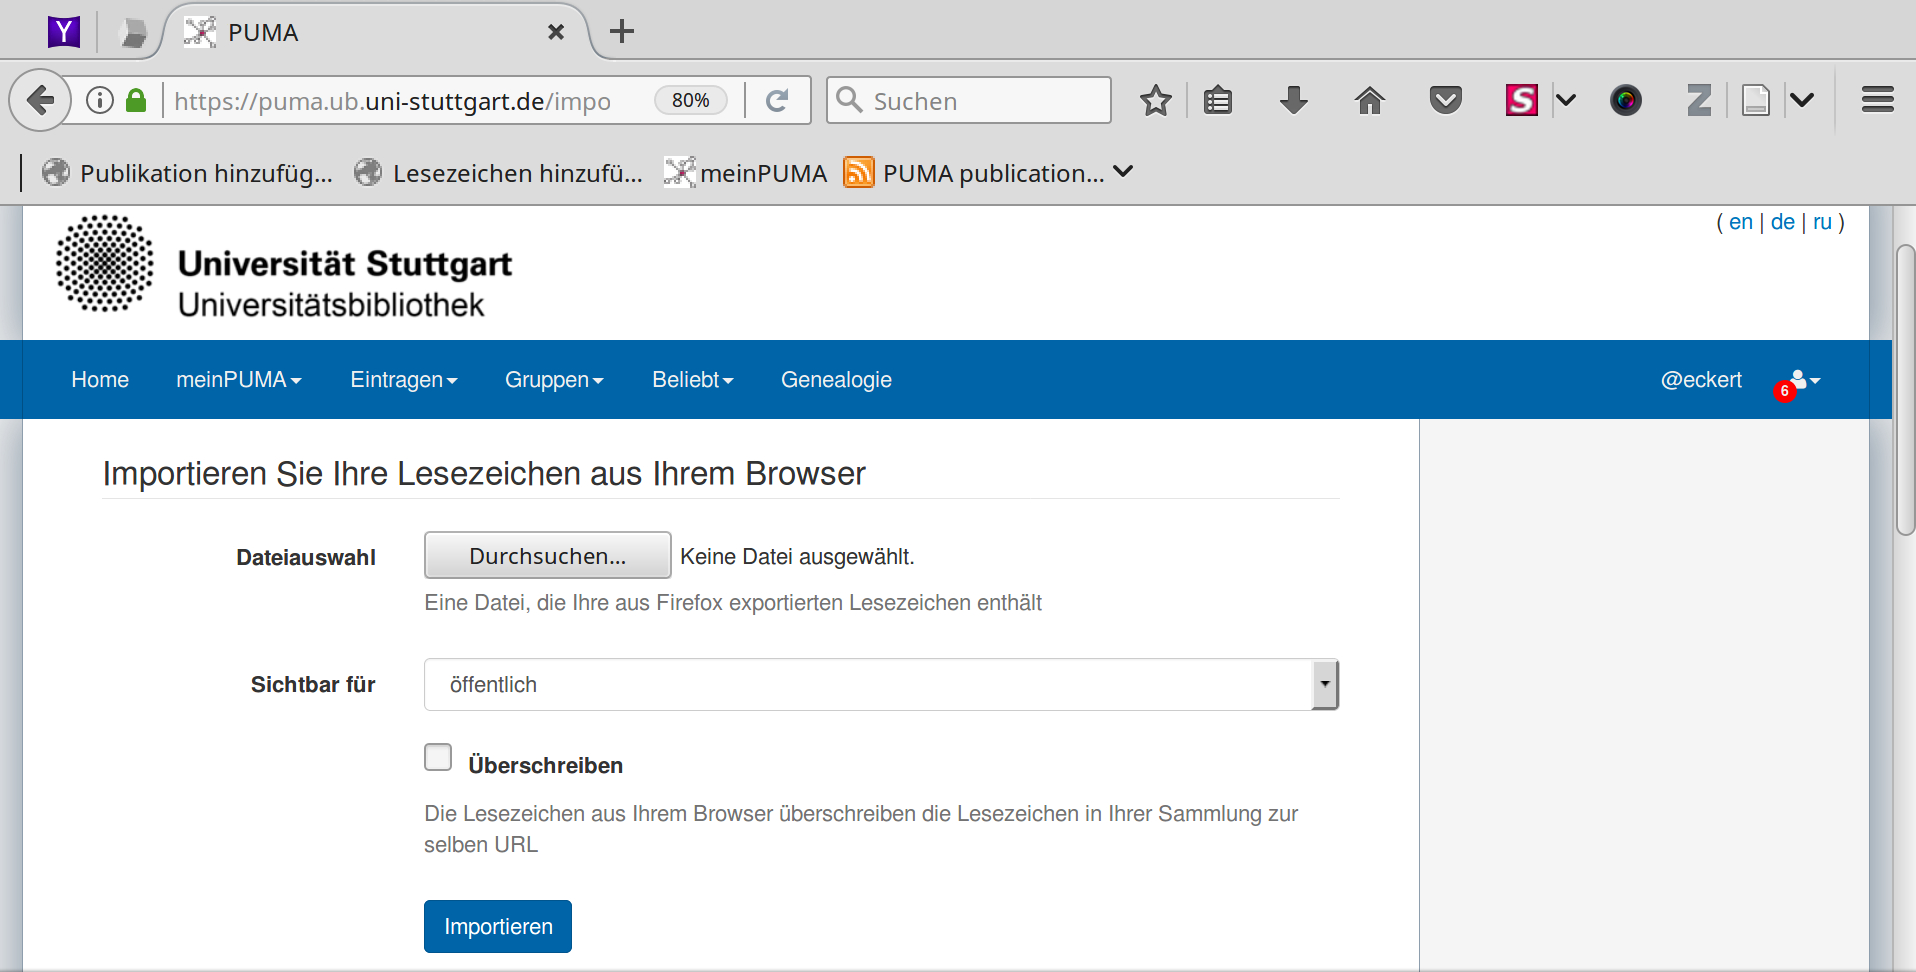
\includegraphics[width=11cm]{Bilder/Kapitel5/HTML-Datei_hochladen}}
 \caption{HTML-Datei hochladen}
 \label{figure017}
\end{figure}
\subsection{Delicious}
Sie möchten Ihre Lesezeichen von Delicious\index{Delicious} nach PUMA importieren. Klicken Sie auf \enquote{Eintragen} und wählen im Dropdown-Menü \enquote{Lesezeichen importieren} aus. Geben Sie unter dem Bereich \enquote{Importieren Sie Ihre Delicious Daten} Ihre Delicious-Nutzerdaten ein. \newline
Legen Sie im darauffolgenden Schritt fest, ob Ihre Delicious Lesezeichen bereits vorhandene Lesezeichen in Ihrer Sammlung mit der selben URL überschreiben sollen.\newline
Sie können im letzten Schritt festlegen, ob Sie Ihre Lesezeichen oder Tag-Bundles importieren möchten. Wenn Sie die Option \enquote{Lesezeichen} wählen, werden zusammen mit Ihren Lesezeichen die dazugehörigen Tags und Sichtbarkeitsdefinitionen mit übernommen.
\newline Klicken Sie abschließend auf \enquote{Importieren} um den Import endgültig durchzuführen.
\begin{figure}[h!]
 \centering
 \fbox{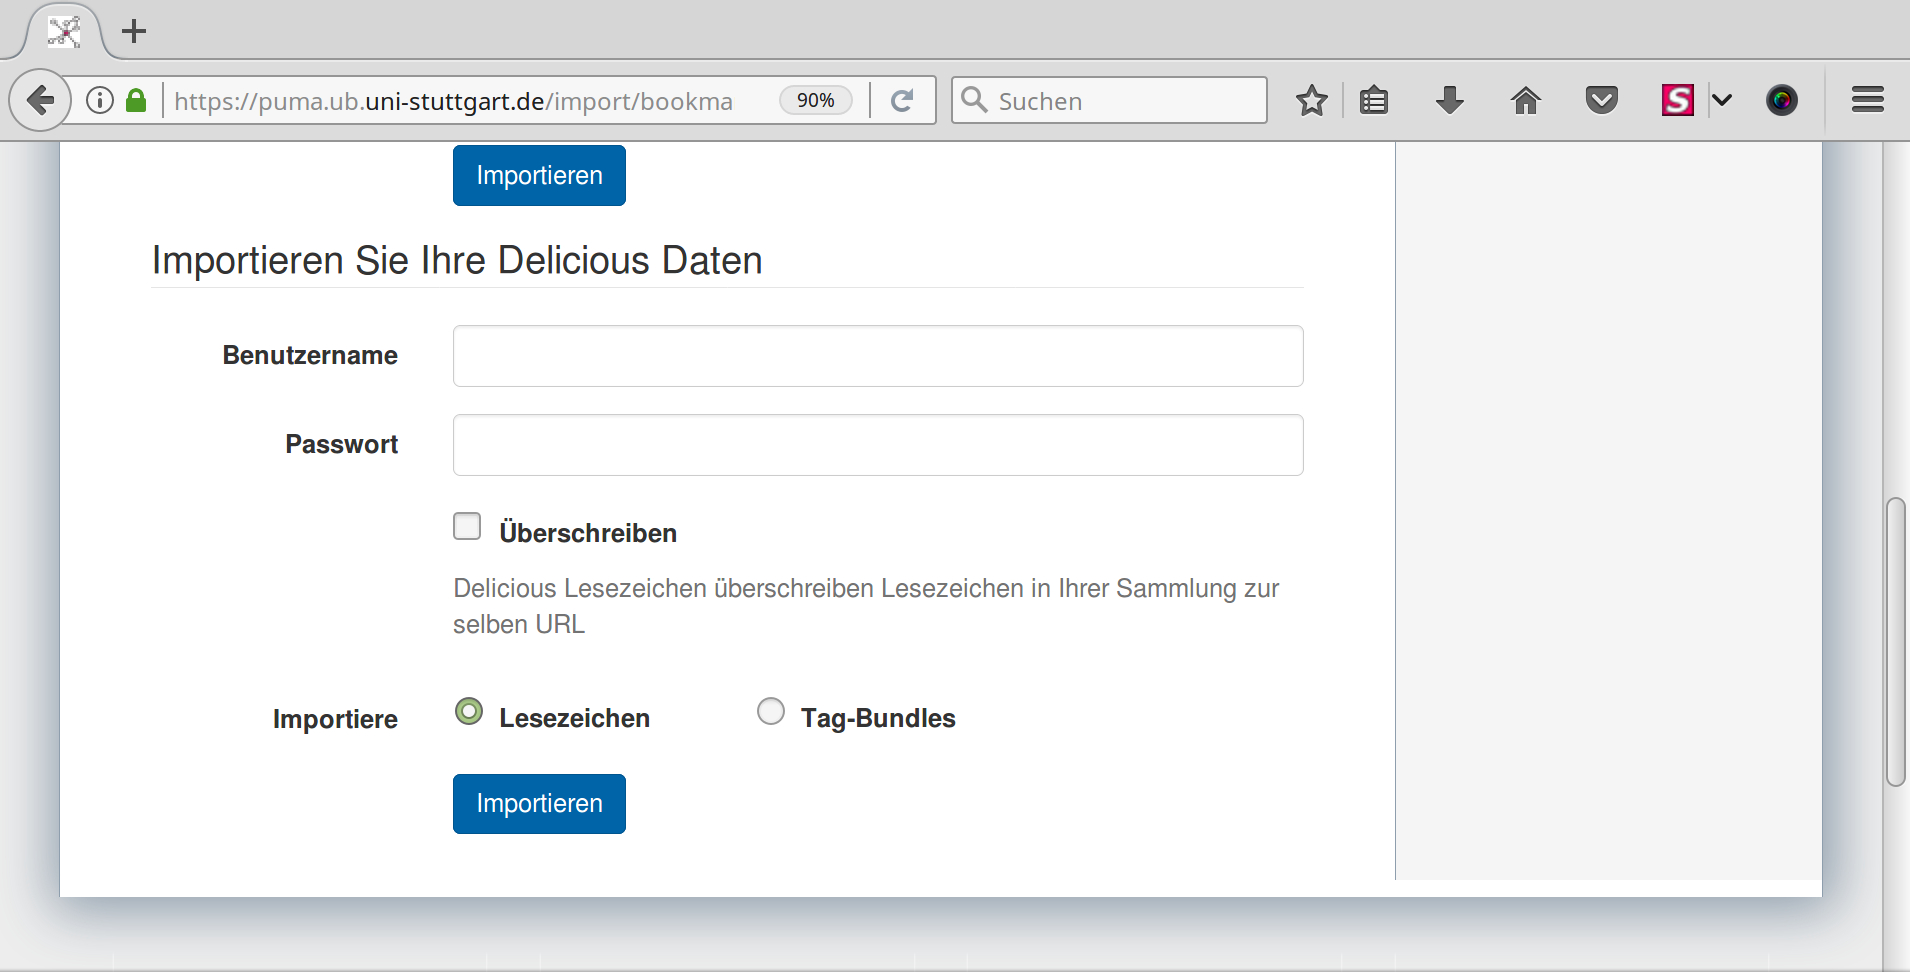
\includegraphics[width=11cm]{Bilder/Kapitel5/Delicious_Daten}}
 \caption{Delicious Daten}
 \label{figure018}
\end{figure} 
\section{Publikationen importieren}
PUMA ermöglicht Ihnen bereits bestehende BibTeX- oder EndNote-Datei hochladen. Vergewissern Sie sich hierbei, dass Sie die korrekte Kodierung gewählt haben. Falls die Datei nur wenige Einträge enthält, können Sie diese auf der folgenden Seite bearbeiten. 
\begin{enumerate}
	\item Klicken Sie auf das Feld \enquote{Durchsuchen} und laden die entsprechende Datei hoch. 
	\item Wählen Sie die Sichtbarkeit aus.
	\item In den \enquote{Erweiterte Einstellungen} können Sie anschließend noch die Datei vor dem Import bearbeiten und festlegen, ob ein älterer Eintrag überschrieben werden soll, wenn der importierte Eintrag die gleiche Publikation referenziert wie ein bereits existierender Eintrag.
	\item Klicken Sie anschließend auf \enquote{Weiter}, um den Eintrag zu vervollständigen und zu speichern.
\end{enumerate}
\begin{figure}[h!]
 \centering
 \fbox{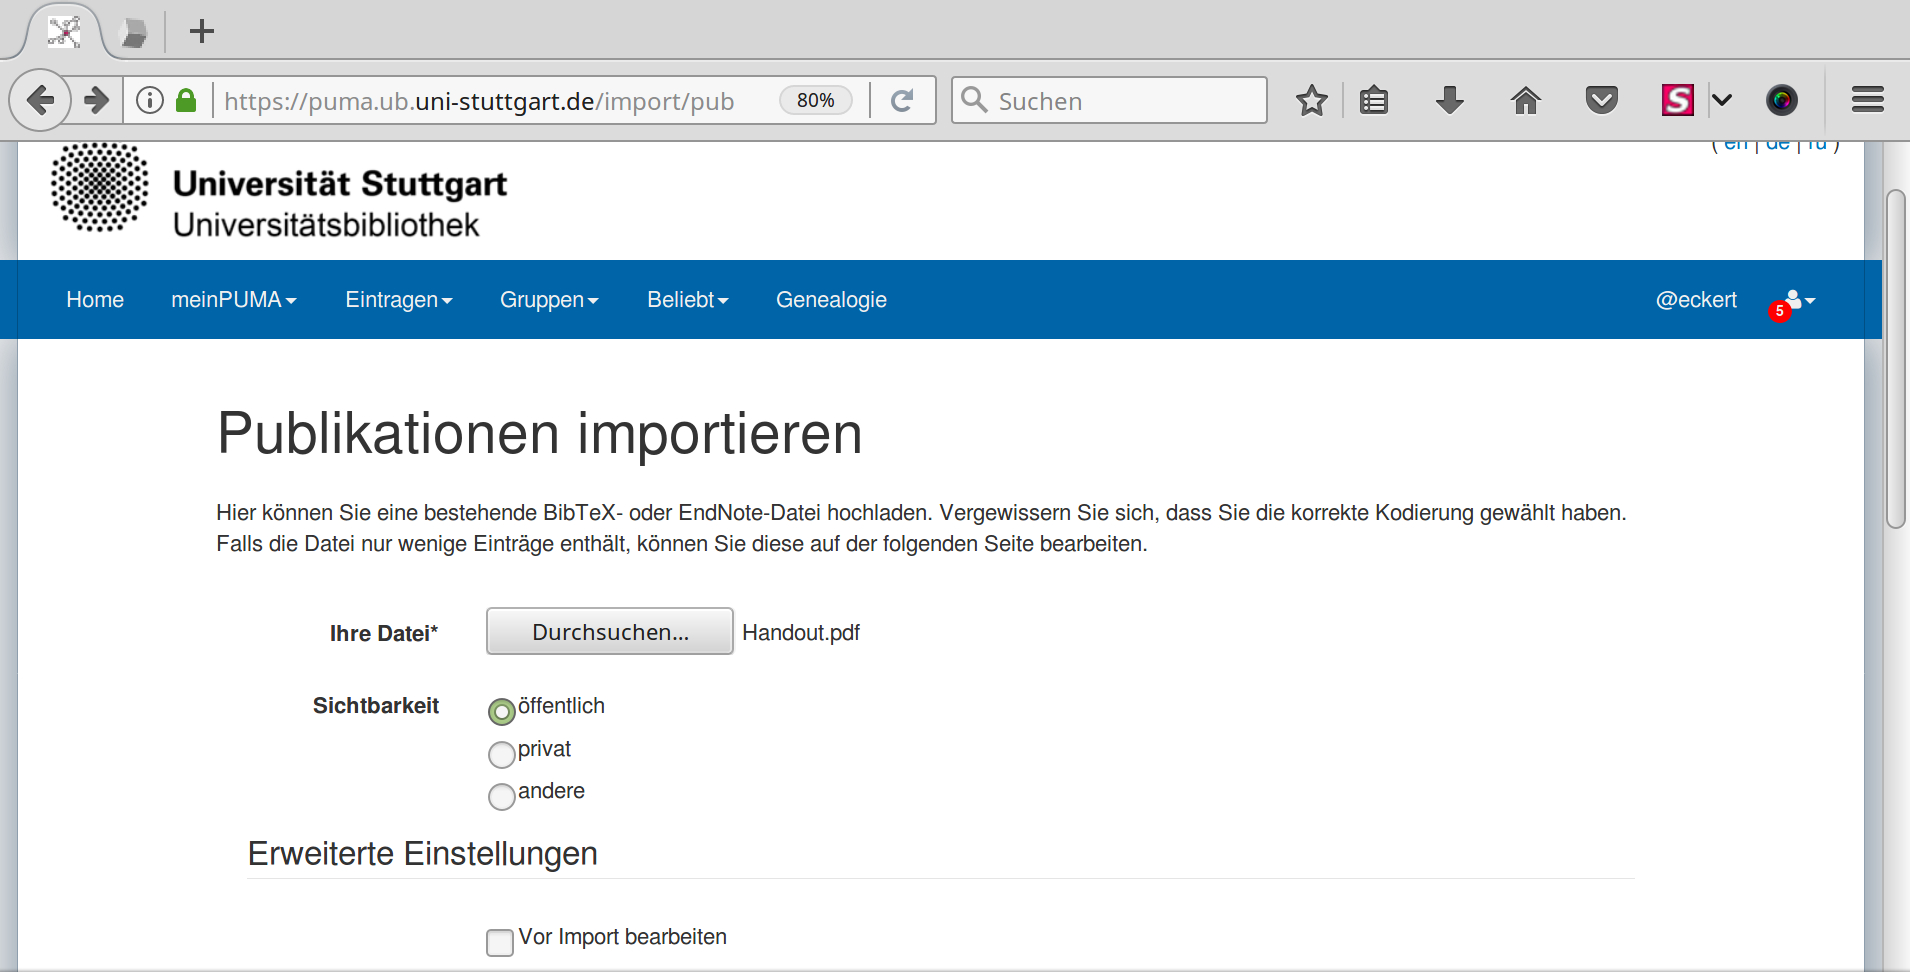
\includegraphics[width=11cm]{Bilder/Kapitel5/Publikationen_importieren}}
 \caption{Publikationen importieren}
 \label{figure019}
\end{figure}  



  
\section{Bookmarklet-Buttons für Ihre Lesezeichen-Leiste}
Die Bookmarklet-Buttons\index{Bookmarklet-Buttons} ermöglichen Ihnen ein schnelles Arbeiten mit PUMA, während Sie im Internet unterwegs sind. Sie vereinfachen Ihnen das Eintragen von Publikationen und Lesezeichen und gelangen mit dem PUMA-Home Bookmarklet-Button direkt zu PUMA. Ziehen Sie die Buttons\footnote{\url{https://puma.ub.uni-stuttgart.de/buttons}} einfach in Ihre Lesezeichen-Leiste und schon können Sie loslegen.
\begin{figure}[h!]
 \centering
 \fbox{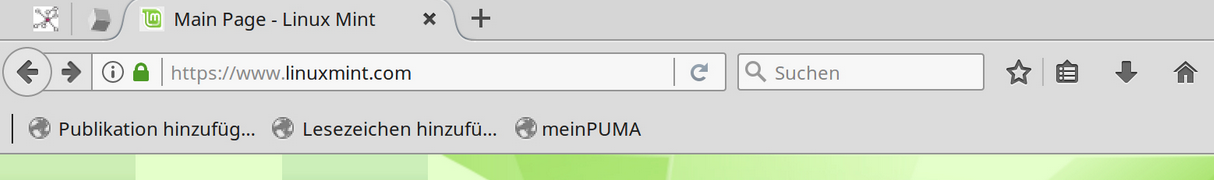
\includegraphics[width=11cm]{Bilder/Kapitel5/Bookmarklet-Buttons}}
 \caption{Bookmarklet-Buttons}
 \label{figure020}
\end{figure} 
\section{PUMA-Browser-ADD-ons\index{Add-ons}}
Erweitern Sie Ihren Browser mit diesem Add-on um drei nützliche PUMA-Schaltflächen: Mit einem Klick zu PUMA, eine Publikation oder ein Lesezeichen speichern.\newline
\begin{enumerate}
\item Klicken Sie rechts oben im Firefox-Browser auf das Menü.
\begin{figure}[h!]
 \centering
 \fbox{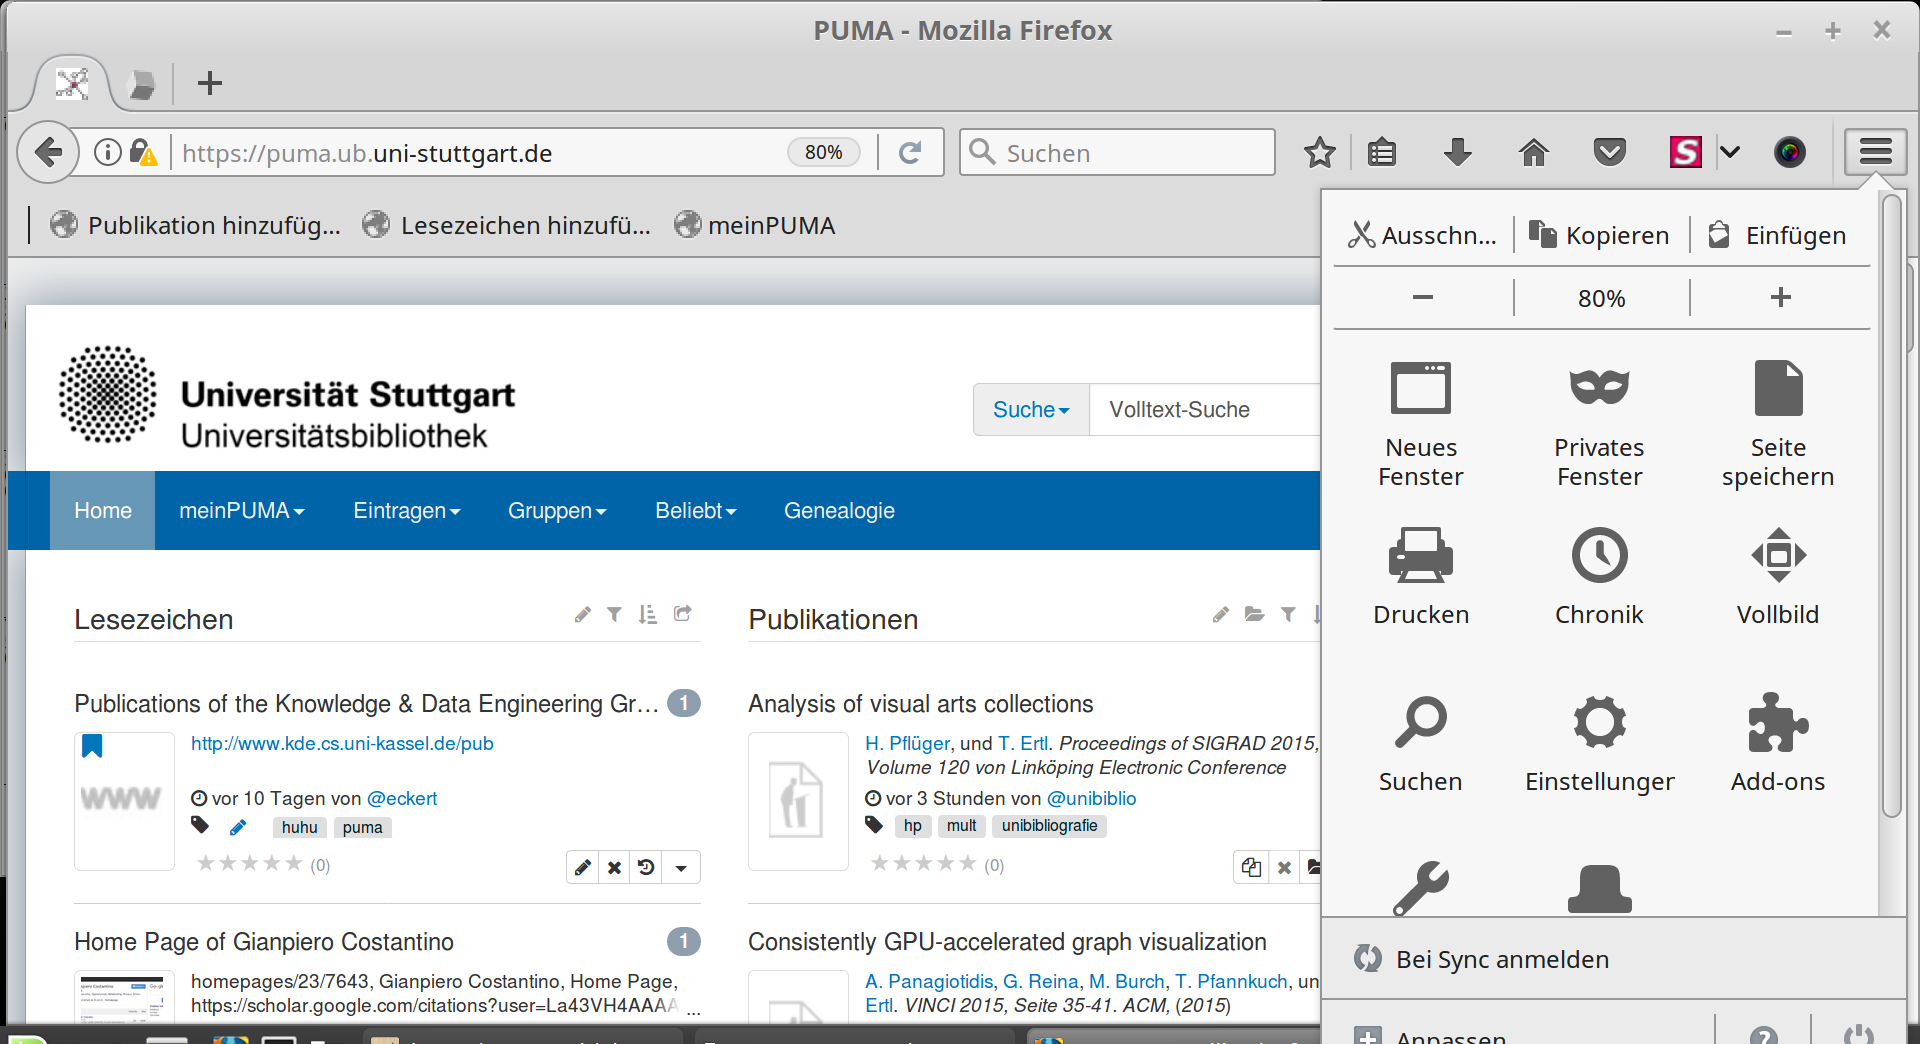
\includegraphics[width=11cm]{Bilder/Kapitel5/Menue_Firefox}}
 \caption{Firefox-Browser}
 \label{figure021}
\end{figure} 
\item Es öffnet sich das Menü, wählen Sie den Reiter \enquote{Add-ons} aus. 
\item Geben Sie in die Suchleiste oben rechts \enquote{puma} ein.
\item Es erscheint das Add-on \enquote{PUMA Buttons}. Installieren Sie die Buttons (Version 1.6.2).
\begin{figure}[h!]
 \centering
 \fbox{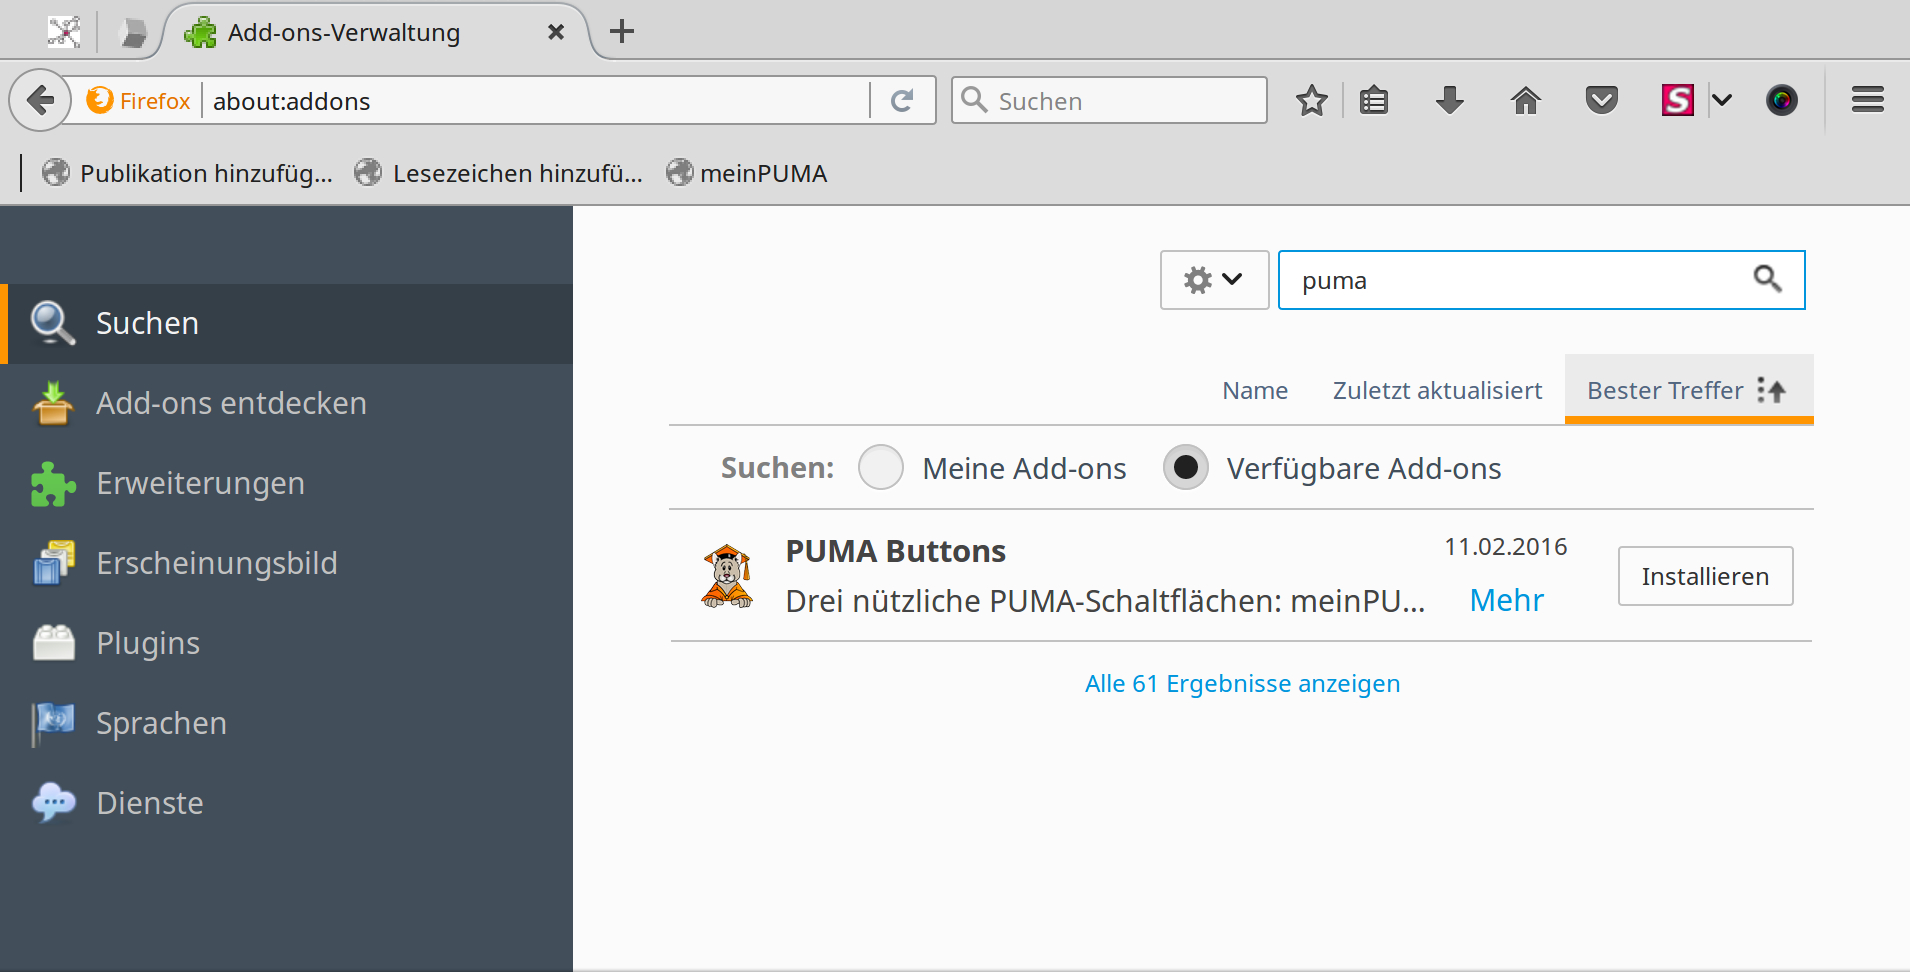
\includegraphics[width=11cm]{Bilder/Kapitel5/PUMA_Buttons}}
 \caption{Puma Buttons}
 \label{figure022}
\end{figure} 
\item Klicken Sie anschließend auf \enquote{mehr} und scrollen auf der Seite runter bis zum Abschnitt \enquote{Instanz wechseln}. 
\item Durch das Klicken auf \enquote{Instanz wechseln} öffnet sich eine Übersicht über alle verfügbaren PUMAs. Wählen Sie  \enquote{UB Stuttgart} aus und speichern Ihre Wahl.
\item Falls die Buttons nicht sofort in der Taskleiste neben dem Menüsymbol  erscheinen, schließen Sie Firefox. Beim erneuten Öffnen des Firefox-Browsers wurden die Buttons eingerichtet.
\end{enumerate}
\section{Ablage}
Die Ablage\index{Ablage} ermöglicht es Ihnen eigene und fremde Publikationen vorzumerken. Sie können so in der Ablage aktuelle Literaturlisten zusammenstellen.
\newline
Publikationen in Ablage aufnehmen: %Screenshot
\begin{enumerate}
    \item Klicken Sie auf das Symbol \enquote{Diese Publikation zur Ablage hinzufügen}.
    \item Die Publikationen gelangen direkt in die Ablage. Zur Ablage gelangen Sie über das Personensymbol.
\end{enumerate}
\begin{figure}[h!]
 \centering
 \fbox{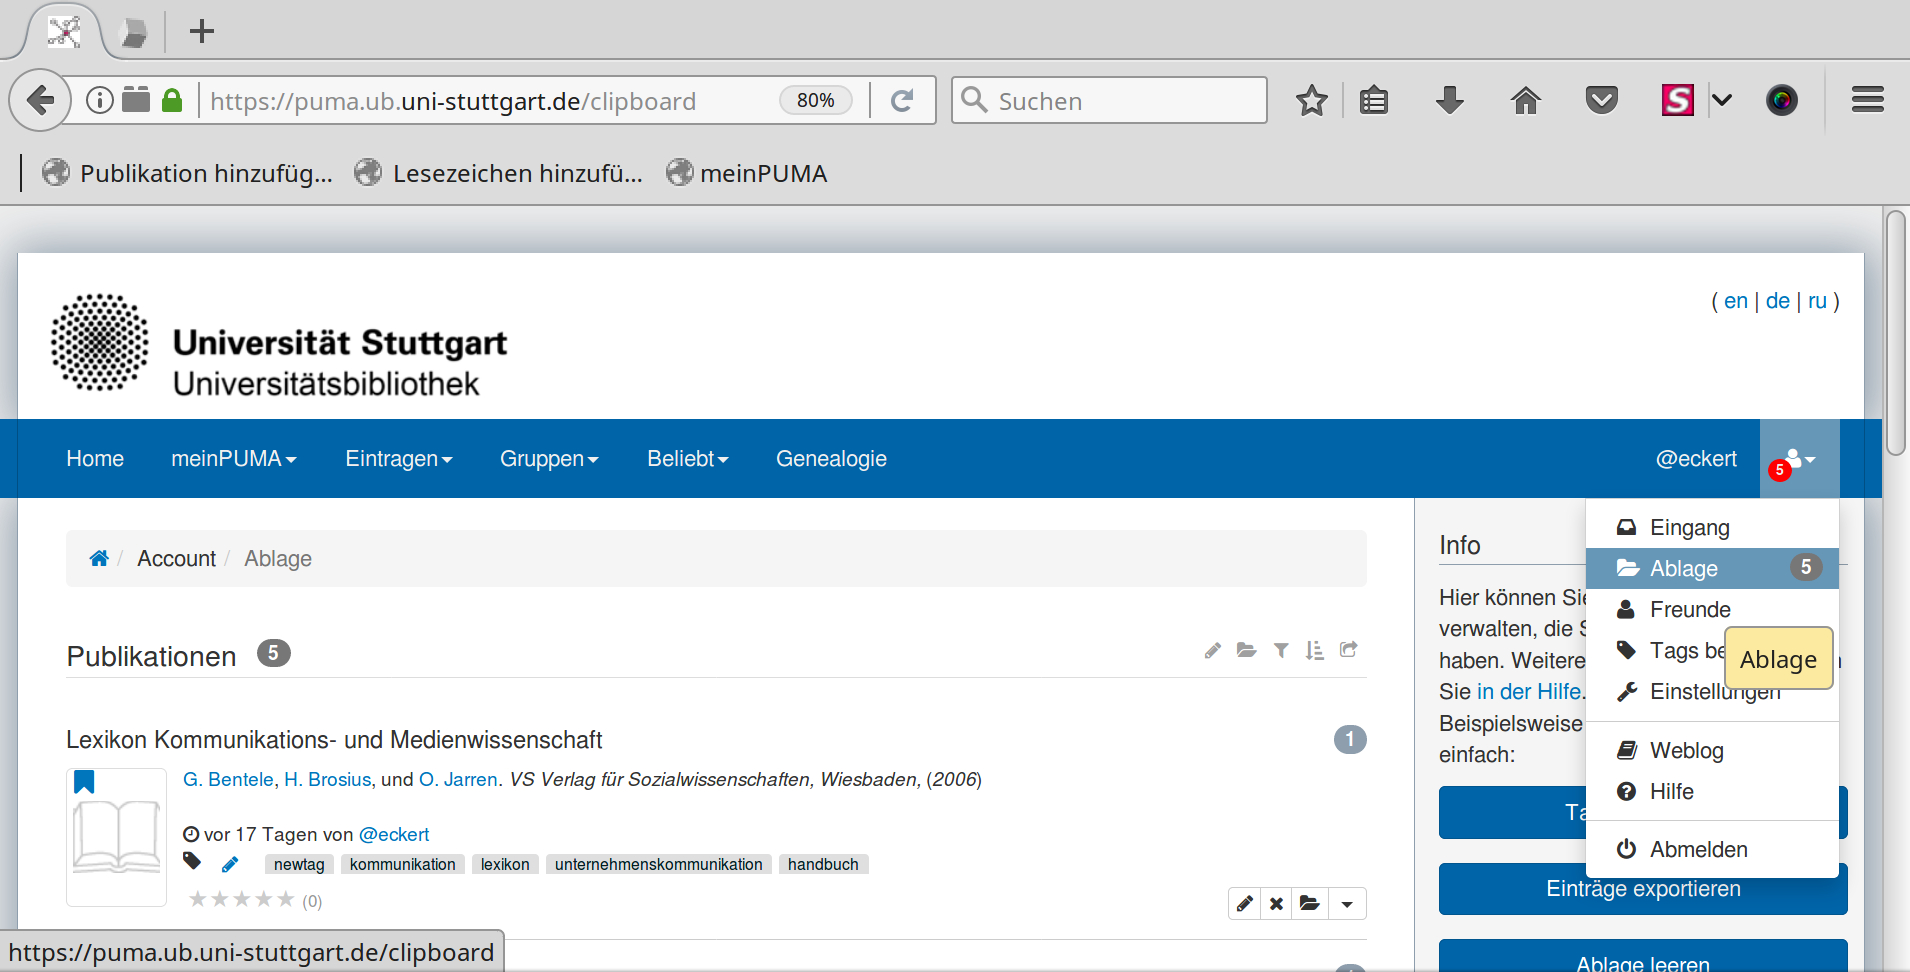
\includegraphics[width=11cm]{Bilder/Kapitel5/Ablage}}
 \caption{Die Ablage}
 \label{figure023}
\end{figure} 
Falls Sie die vorgemerkten Publikationen nicht mehr in der Ablage haben möchten können Sie diese löschen, indem Sie auf das schwarze \enquote{X} (diese Publikation aus Ihrer Sammlung löschen) klicken.\newline
%\begin{wrapfigure}{l}{5cm}
\begin{mdframed}[style=mdfexample1,frametitle={\texttt{ACHTUNG}},backgroundcolor=gray!40]\texttt{Wenn Sie die Publikation in der Ablage löschen ist diese gleichzeitig auch in Ihrer Sammlung gelöscht und kann nicht wiederhergestellt werden.}
\end{mdframed}
%\end{wrapfigure}

Eine andere Möglichkeit ist das Leeren der Ablage. Dies erreichen Sie, indem Sie auf der rechten Seite auf das blaue Feld \enquote{Ablage leeren} klicken. In diesem Fall werden die Publikationen aus der Ablage entfernt, sind aber in Ihrer Sammlung noch vorhanden.
\section{Freischalten erweiterter Funktionen}
Bei PUMA gibt es die Unterscheidung zwischen einfachen\index{Funktionen!Einfache} und erweiterten Funktionen\index{Funktionen!Erweiterte}. In den Grundeinstellungen stehen jedem Nutzer, bei dessen Anmeldung bei PUMA, die einfachen Funktionen zur Verfügung. Durch das Freischalten der erweiterten Funktionen kommen weitere Funktionen hinzu, sodass Sie mehr Möglichkeiten haben, PUMA zu nutzen.  Wenn Sie die erweiterten Funktionen freischalten möchten, gehen Sie wie folgt vor:
\begin{enumerate}
    \item Klicken Sie auf das Personensymbol. Ein Dropdown-Menü öffnet sich, klicken Sie auf \enquote{Einstellungen}.
    \item Es öffnet sich die Einstellungs-Seite. Klicken Sie oben auf den Reiter \enquote{Einstellungen}.
    \item Unter dem Bereich \enquote{Layouts Ihrer Tagbox und Ihrer Eintragslisten} befindet sich das Feld \enquote{Erscheinungsbild}. Sie können nun zwischen den Standardeinstellungen \textit{Erweitert} (Alle Optionen werden stets angezeigt) oder \textit{Einfach} (Einige \enquote{Experten}-Optionen werden standardmäßig nicht angezeigt) wählen.
    \begin{figure}[h!]
 \centering
 \fbox{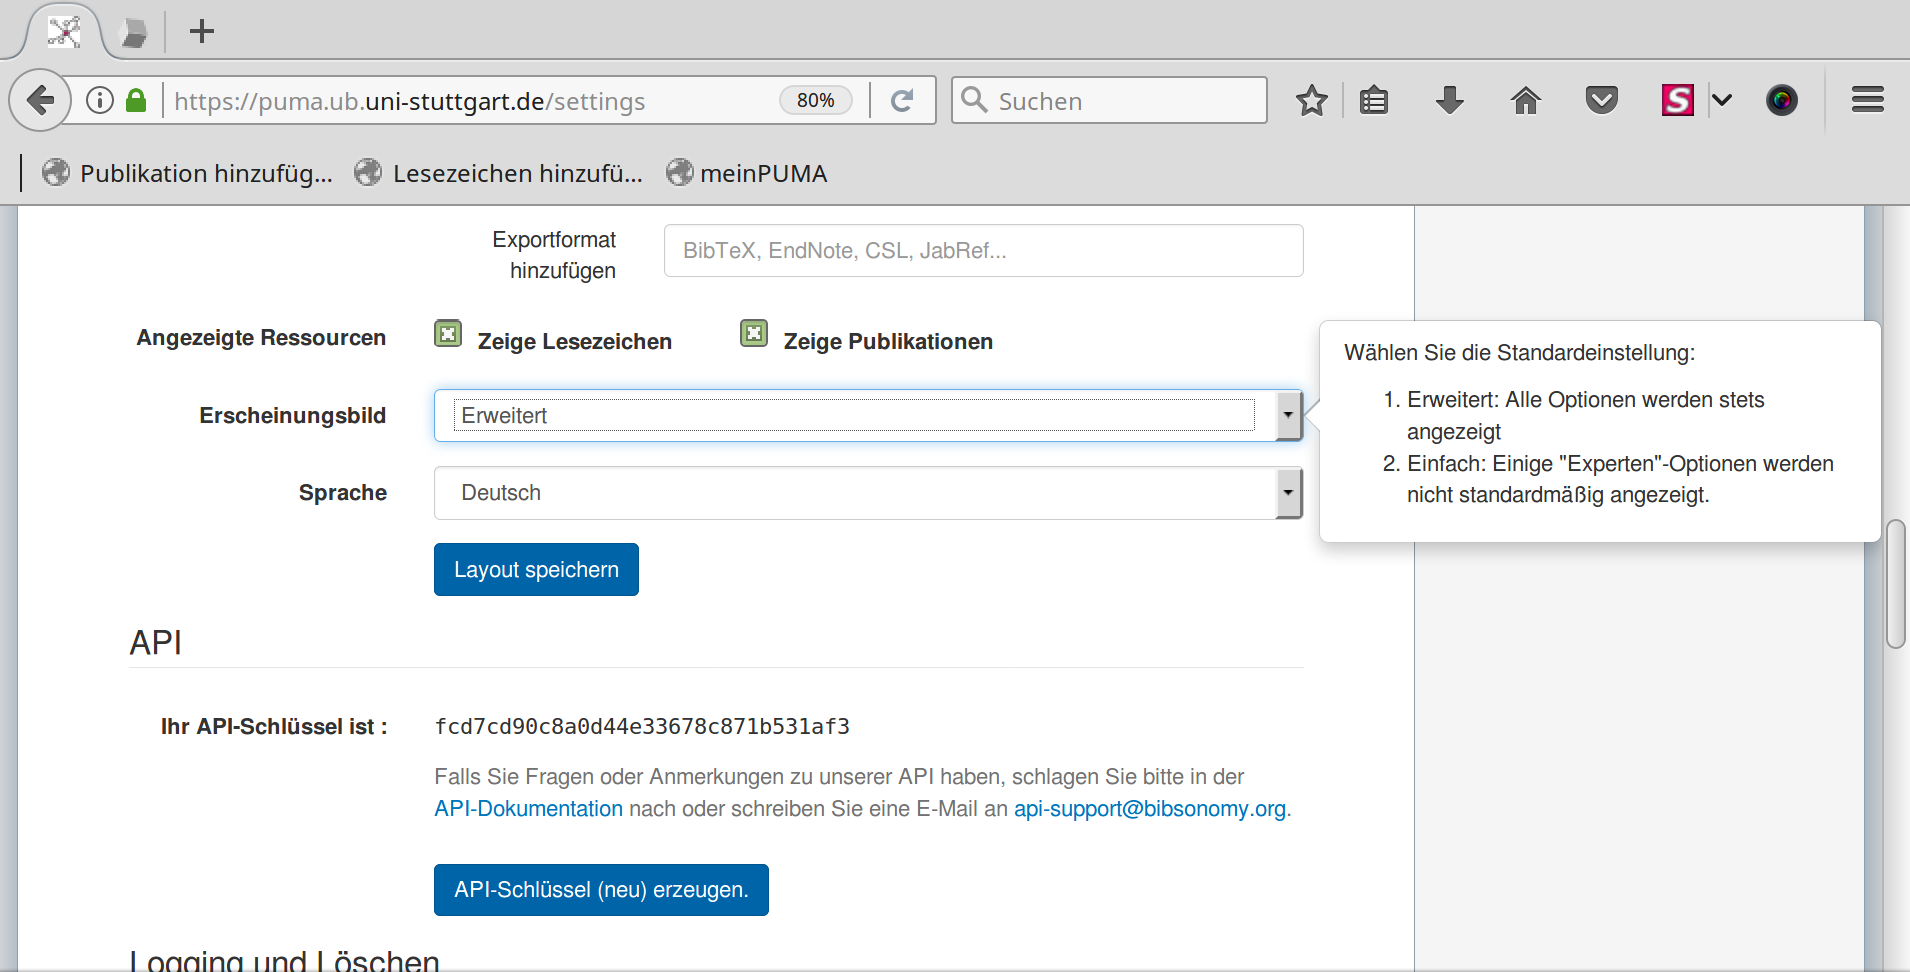
\includegraphics[width=11cm]{Bilder/Kapitel5/Erweiterte_Funktionen}}
 \caption{Erweiterte Funktionen}
 \label{figure024}
\end{figure} 
    \item Klicken Sie anschließend auf \enquote{Layout speichern}, um Ihre Änderung zu sichern.
\end{enumerate}